%% Copernicus Publications Manuscript Preparation Template for LaTeX Submissions
%% ---------------------------------
%% This template should be used for the following class files: copernicus.cls, copernicus2.cls, copernicus_discussions.cls
%% The class files, the Copernicus LaTeX Manual with detailed explanations regarding the comments
%% and some style files are bundled in the Copernicus Latex Package which can be downloaded from the different journal webpages.
%% For further assistance please contact the Publication Production Office (production@copernicus.org).
%% http://publications.copernicus.org


%% Differing commands regarding the specific class files are highlighted.


%% copernicus.cls
\documentclass[gmd,manuscript]{copernicus}
%\documentclass[gmdd, hvmath, online]{copernicus_discussions}

% A few handy shortcuts
\newcommand{\uf}{\ensuremath{\widetilde{u}}}
\newcommand{\vf}{\ensuremath{\widetilde{v}}}
\newcommand{\thetaf}{\ensuremath{\widetilde{\theta}}}
\newcommand{\phif}{\ensuremath{\widetilde{\phi}}}

\begin{document}

\linenumbers
%\raggedbottom

\title{MicroHH 1.0: a computational fluid dynamics code for direct numerical simulation and large-eddy simulation of atmospheric boundary layer flows}

\author[1,2]{Chiel C. van Heerwaarden}
\author[1,2]{Bart J. H. van Stratum}
\author[3]{Thijs Heus}
\author[4]{Jeremy A. Gibbs}
\author[5]{Evgeni Fedorovich}
\author[2]{Juan-Pedro Mellado}

\affil[1]{Meteorology and Air Quality Group, Wageningen University, Wageningen, The Netherlands}
\affil[2]{Max Planck Institute for Meteorology, Hamburg, Germany}
\affil[3]{Cleveland State University, Cleveland, OH, USA}
\affil[4]{Department of Mechanical Engineering, University of Utah, UT, USA}
\affil[5]{University of Oklahoma, Norman, OK, USA}

%% The [] brackets identify the author to the corresponding affiliation, 1, 2, 3, etc. should be inserted.

\runningtitle{MicroHH 1.0}

\runningauthor{van Heerwaarden et al.}

\correspondence{Chiel van Heerwaarden\\ (chiel.vanheerwaarden@wur.nl)}

\received{}
\pubdiscuss{} %% only important for two-stage journals
\revised{}
\accepted{}
\published{}

%% These dates will be inserted by the Publication Production Office during the typesetting process.

\firstpage{1}

\maketitle  %% Please note that for the copernicus2.cls this command needs to be inserted after \abstract{TEXT}

\begin{abstract}
This paper describes MicroHH 1.0, a new and open source (\url{www.microhh.org}) computational fluid dynamics code for the simulation of turbulent flows in the atmosphere. It is primarily made for direct numerical simulation, but also supports large-eddy simulation (LES). The paper covers the description of the governing equations, their numerical implementation, and the parametrizations included in the code. Furthermore, the paper presents the validation of the dynamical core in the form of convergence and conservation tests, and comparison of simulations of channel flows and slope flows against well-established test cases. The full numerical model, including the associated parametrizations for LES, has been tested for a set of cases under stable and unstable conditions, under the Boussinesq and anelastic approximation, and with dry and moist convection under stationary and time-varying boundary conditions. The paper presents performance tests showing good scaling from 256 to 32,768 processes. The Graphical Processing Unit (GPU)-enabled version of the code can reach a speedup of more than an order of magnitude for cases that fit in the memory of a single GPU.
\end{abstract}

\introduction  %% \introduction[modified heading if necessary]
In this paper we present a description of MicroHH 1.0, a new Computational Fluid Dynamics code for the simulation of turbulent flows in doubly periodic domains, with a focus on those in the atmosphere. MicroHH is designed for the direct numerical simulation (DNS) technique, but also supports the large-eddy simulation (LES) technique. Its applications range from neutral channel flows to cloudy atmospheric boundary layers in large domains. MicroHH is written in C++ and the Graphical Processing Units-enabled parts of the code in CUDA. The simulation algorithms have been designed and are written from scratch with the goal to create a fast and highly parallel code that is able to run on machines with more than 10,000 cores. This is a key requirement for the code to be able to perform DNS at very high Reynolds numbers, or to do LES in domains that approach the synoptic scales (beyond 1000 km). We decided to start from scratch, in order to be able to use C++ and its extensive possibilities in object oriented- and metaprogramming. Furthermore, the implementation of a dynamical core that is fully fourth-order in space, which is very beneficial for DNS, but to retain the option to switch to second-order accuracy for LES, required a new code design.

Even though we started from scratch, many of the ideas are the results of our experiences with other codes. Here, DALES \citep{Heus2010}, UCLA-LES \citep{Stevens2005}, and PALM \citep{Maronga2015}, deserve a reference as MicroHH could not have been possible without those.

This paper is built up as following: in Sect. \ref{sec:dyncore}, we provide a full description of the governing equations of the dynamical core, and their numerical implementation is discussed in Sect. \ref{sec:dyncorediscrete}. Subsequently, in Sect. \ref{sec:parametrizations} we present the parameterizations and their underlying assumptions. Section \ref{sec:technical} discusses the technical details of the code, and Sections \ref{sec:running} and \ref{sec:output} explain how to run the model and which output is generated. This is followed by a series of model tests on the validity and accuracy of the dynamical core in Sect. \ref{sec:tests}, and a series of more applied atmospheric flow cases based on previous studies (Sect. \ref{sec:validation_atmos}). Hereafter, the parallel performance is evaluated (Sect. \ref{sec:performance}). Then, an overview of published work with MicroHH is presented (Sect. \ref{sec:published}), followed by the future plans (Sect. \ref{sec:future}) and the concluding remarks (Sect. \ref{sec:conclusion}), there is a short description where to get MicroHH, and where to find its tutorials and a selection of visualisations (Sect. \ref{sec:howto}).

\section{Dynamical core: governing equations}\label{sec:dyncore}
The dynamical core of MicroHH solves the conservation equations of mass, momentum, and energy under the anelastic approximation \citep{Bannon1996}. Under this approximation, the state variables density, pressure, and temperature are described as small fluctuations (denoted with a prime in this paper) from corresponding vertical reference profiles (denoted with subscript zero) that are functions of height only. This form of the approximation directly simplifies to the Boussinesq approximation if the reference density $\rho_0 (z)$ is taken to be constant with height $z$. Consequently, MicroHH does not need separate implementations of Boussinesq and anelastic approximations. To facilitate the subsequent discussion of the conservation equations, we define the scale height for density $H_\rho$ based on the reference density profile
\begin{eqnarray}
H_{\rho} & \equiv & \left( \dfrac{1}{\rho_0} \dfrac{d \rho_0}{dz} \right)^{-1}.
\end{eqnarray}

\subsection{Conservation of mass}
The conservation of mass is formulated using Einstein summation as
\begin{eqnarray}
\dfrac{\partial \rho_0 u_i}{\partial x_i} & = & \rho_0 \dfrac{\partial u_i}{\partial x_i} + \rho_0 w H_{\rho}^{-1} = 0, \label{eq:consmassa}
\end{eqnarray}
where $u_i$ is the velocity vector $(u,v,w)$ and $x_i$ is the position vector $(x,y,z)$. This formulation conserves the reference mass, as density perturbations are ignored in the equation \citep{Lilly1996}.

Under the Boussinesq approximation ($H_{\rho}~\rightarrow~\infty$), Eq. \ref{eq:consmassa} simplifies to conservation of volume
\begin{eqnarray}
\dfrac{\partial u_i}{\partial x_i} & = & 0. \label{eq:consmassb}
\end{eqnarray}

\subsection{The equation of state and conservation of momentum}
The equation of state under the anelastic approximation is (see \citet{Bannon1996} for its derivation)
\begin{eqnarray}
\dfrac{\theta_v'}{\theta_{v0}} & = & \dfrac{p'}{\rho_0 g H_{\rho}} - \dfrac{\rho'}{\rho_0},\label{eq:statea}
\end{eqnarray}
where $\theta_v^\prime$ is the perturbation virtual potential temperature, $\theta_{v0}$ the reference virtual potential temperature, $p^\prime$ is the perturbation pressure, $g$ is the gravity acceleration, and $\rho^\prime$ is the perturbation density.

The corresponding momentum equation is written in the flux form, in order to assure momentum conservation. The hydrostatic balance $dp_0 / dz~=~-\rho_0 g$ has been subtracted and Eq. \ref{eq:statea} has been used to introduce potential temperature as the buoyancy variable to formulate the conservation of momentum as
\begin{eqnarray}
\nonumber \dfrac{\partial u_i}{\partial t} & = & - \dfrac{1}{\rho_0} \dfrac{\partial \rho_0 u_i u_j}{\partial x_j} 
- \dfrac{\partial}{\partial x_i}\left(\dfrac{p'}{\rho_0}\right) \\
& + & \delta_{i3} g \dfrac{\theta_v'}{\theta_{v0}} + \nu \dfrac{\partial^2 u_i}{\partial x_j^2} + F_i,\label{eq:consmoma}
\end{eqnarray}
where $\delta$ is the Kronecker delta, $\nu$ the kinematic viscosity, and vector $F_i$ represents external forces resulting from parameterizations or large-scale forcings. As \citet{Bannon1996} showed, this formulation is energy-conserving in the sense that there is a consistent transfer between kinetic and potential energy.

Under the Boussinesq approximation, the two equations simplify to
\begin{eqnarray}
\nonumber \dfrac{\partial u_i}{\partial t} & = & - \dfrac{\partial u_i u_j}{\partial x_j} - \dfrac{1}{\rho_0}\dfrac{\partial p^\prime}{\partial x_i} \\
& + & \delta_{i3} g \dfrac{\theta_v'}{\theta_{v0}} + \nu \dfrac{\partial^2 u_i}{\partial x_j^2} + F_i \label{eq:consmomb},\\
\dfrac{\theta_v'}{\theta_{v0}} & = & - \dfrac{\rho'}{\rho_0}\label{eq:stateb}.
\end{eqnarray}

\subsection{Pressure equation}
The equation to acquire the pressure is diagnostic, because density fluctuations are neglected in the mass conservation equation under the anelastic approximation (Eq. \ref{eq:consmassa}). To simplify the notation, we define a function $f \left( u_i \right)$ that contains all right-hand side terms of Eq. \ref{eq:consmoma}, except the pressure gradient. To arrive at the equation that allows us to solve for the pressure, we multiply the equation with the base density $\rho_0$ and take its divergence. Conservation of mass ensures that the tendency term vanishes, and an elliptic equation for pressure remains
\begin{eqnarray}
\dfrac{\partial}{\partial x_i} 
\left[ \rho_0 \dfrac{\partial}{\partial x_i} \left( \dfrac{p'}{\rho_0} \right) \right] & = &
\dfrac{\partial \rho_0 f \left( u_i \right)}{\partial x_i}.\label{eq:presa}
\end{eqnarray}
Under the Boussinesq approximation the equation simplifies to
\begin{eqnarray}
\dfrac{\partial^2}{\partial x_i^2} \left( \dfrac{p'}{\rho_0} \right) & = &
\dfrac{\partial f \left( u_i \right)}{\partial x_i}.\label{eq:presb}
\end{eqnarray}
In Sect. \ref{sec:dyncorediscrete} we explain how these equations are solved numerically.

\subsection{Conservation of an arbitrary scalar}
The conservation equation of an arbitrary scalar $\phi$ is written in flux form
\begin{eqnarray}
\dfrac{\partial \phi}{\partial t} & = & - \dfrac{1}{\rho_0} \dfrac{\partial \rho_0 u_j \phi}{\partial x_j} +
\kappa_\phi \dfrac{\partial^2 \phi}{\partial x_j^2} + S_\phi, \label{eq:consscal}
\end{eqnarray}
where $\kappa_\phi$ is the diffusivity of the scalar, and $S_\phi$ represents sources and sinks of the variable.

\subsection{Conservation of energy}\label{sec:dyncore_energy}
\label{sec:conservation_of_energy}
MicroHH provides multiple options for the energy conservation equation. The conservation equation for  potential temperature for dry dynamics $\theta$ can be written as
\begin{eqnarray}
\dfrac{\partial \theta}{\partial t} & = & - \dfrac{1}{\rho_0} \dfrac{\partial \rho_0 u_j \theta}{\partial x_j} + \kappa_\theta \dfrac{\partial^2 \theta}{\partial x_j^2} + \dfrac{\theta_0}{\rho_0 c_p T_0} Q,\label{eq:consthermo}
\end{eqnarray}
where $\kappa_\theta$ is the thermal diffusivity for heat, and $Q$ represents external sources and sinks of heat. A second option for moist dynamics is available. This has an identical conservation equation, but with liquid water potential temperature $\theta_l$ (moist dynamics), rather than $\theta$ as the conserved variable (see Sect. \ref{sec:thermo} for details). In the dry mode, the Brunt-Vaissala frequency $N$ is defined as $N^2 \equiv \left(g/\theta_0\right) \left( \partial \theta/\partial z \right)$, whereas in the moist dynamics $N^2 \equiv \left(g/\theta_{v0}\right) \left( \partial \theta_v/\partial z \right)$.

A third, more simplified mode, is available for dry dynamics under the Boussinesq approximation. Here, the equation of state can be eliminated and the conservation of momentum and energy can be written using buoyancy $b \equiv -(g/\rho_0)\rho^\prime$ as
\begin{eqnarray}
\dfrac{\partial u_i}{\partial t} + \dfrac{\partial u_i u_j}{\partial x_j} & = & 
- \dfrac{1}{\rho_0}\dfrac{\partial p'}{\partial x_i} + \delta_{i3} b + \nu \dfrac{\partial^2 u_i}{\partial x_j^2}\label{eq:consmombsimp},\\
\dfrac{\partial b}{\partial t} + \dfrac{\partial b u_j}{\partial x_j} & = & 
\kappa_b \dfrac{\partial^2 b}{\partial x_j^2} + Q_b \label{eq:consbsimp}.
\end{eqnarray}
with $\kappa_b$ being the diffusivity for buoyancy, and $Q_b$ is an external buoyancy source. In this mode, $N$ is defined as $N^2 \equiv \partial b/\partial z$.

With a slight modification to the previous set of equations, it is possible to study slope flows in periodic domains. If we introduce a slope $\alpha$ (positive anticlockwise, thus $x$-axis pointing upslope, see \citet{Fedorovich2009}, their Fig. 1) in the $x$-direction, take the proper gravity vector, and define the buoyancy as $b \equiv -(g/\rho_0)\rho^\prime - N_0^2 z$, with $N_0^2$ as a prescribed background buoyancy profile, the set of Eqs. \ref{eq:consmombsimp} and \ref{eq:consbsimp} becomes
\begin{eqnarray}
\dfrac{\partial u}{\partial t} + \dfrac{\partial u_j u}{\partial x_j} & = & 
- \dfrac{1}{\rho_0}\dfrac{\partial p'}{\partial x} + \sin(\alpha) b + \nu \dfrac{\partial^2 u}{\partial x_j^2}\label{eq:consuslope},\\
\dfrac{\partial w}{\partial t} + \dfrac{\partial u_j w}{\partial x_j} & = & 
- \dfrac{1}{\rho_0}\dfrac{\partial p'}{\partial z} + \cos(\alpha) b + \nu \dfrac{\partial^2 w}{\partial x_j^2}\label{eq:conswslope},\\
\dfrac{\partial b}{\partial t} + \dfrac{\partial b u_j}{\partial x_j} & = & 
\kappa_b \dfrac{\partial^2 b}{\partial x_j^2} - \left (u\,\sin(\alpha) + w\,\cos(\alpha) \right) N_0^2 + Q_b.\label{eq:consbslope}
\end{eqnarray}
where the evolution equation of $v$ is omitted as it contains no changes. In this formulation, $N$ is defined as $N^2 \equiv \partial b/\partial z + N_0^2$.

\section{Dynamical core: numerical implementation}\label{sec:dyncorediscrete}
\subsection{Grid}\label{sec:grid}
MicroHH is discretized on a staggered Arakawa C-grid, where the scalars are located in the center of a grid cell and the three velocity components at the faces. The code can work with stretched grids in the vertical dimension. The grid is initialized from a vertical profile that contains the heights of the cell centres. The locations of the faces are determined consistently with the spatial order of the interpolations that are described in Sect. \ref{sec:buiding_blocks}. All spatial operators in the model, such as the advection and diffusion, default to the same order as the grid, and can be overriden according to the user's wishes (see Sect. \ref{sec:running}).

There is the option to apply a uniform translation velocity to the grid, thus to let the grid move with the flow. This so-called Galilean transformation is allowed as the Navier-Stokes equations are invariant under translation. It has the potential to allow for larger time steps and to increase the accuracy of simulations.

\subsection{Three-dimensional fields}
In order to solve the governing equations, MicroHH generates at initialization three-dimensional fields of the prognostic variables. These are the three velocity components (Eqs. \ref{eq:consmoma} or \ref{eq:consmomb}), and the thermodynamic variables (Eqs. \ref{eq:consthermo}, \ref{eq:consbsimp}, or \ref{eq:consbslope}). Furthermore, the user has the option to define additional passive scalars (Eq. \ref{eq:consscal}). Each of the prognostic fields has an additional three-dimensional field assigned to store its tendency (see Sect. \ref{sec:time_integration}). Furthermore, a diagnostic field is assigned for the pressure, as well as three or four additional ones for intermediate computations. Newly implemented physical parameterizations have the option to request additional three-dimensional fields at initialization of the specific parameterization.

The generation of turbulence requires perturbations to the initial fields. MicroHH has to option to superimpose perturbations in a user-specified layer on any of the prognostic variables. These perturbations can be random noise of which the amplitude and location can be controlled, as well as two-dimensional rotating vortices with an axis aligned with the $x$- or $y$-dimension. The former option is the most commonly used method to start convective turbulence, whereas the latter is the default for neutral or stably-stratified flows that develop turbulence more easily from larger perturbations.

\subsection{Time integration}\label{sec:time_integration}
The prognostic equations are solved using low-storage Runge-Kutta time integration schemes. Such schemes require two fields per variable: one that contains the actual value, which we denote with $\phi$ in this section, and one that represents the tendencies, denoted with $\delta \phi$. The code provides two options: a three-stage third-order scheme \citep{Williamson1980} and a five-stage fourth-order scheme \citep{Carpenter1994}. Both can be written in the same generic form in semi-discrete formulation as
\begin{eqnarray}
\left( \delta \phi \right)_n & = & f \left( \phi_n \right) + a_n \left( \delta \phi \right)_{n-1} \\
\phi_{n+1} & = & \phi_n + b_n \Delta t \left( \delta \phi \right)_{n},
\end{eqnarray}
where $f$ is a function that represents the computation of all right-hand side terms, $a_n$ and $b_n$ are the coefficients for the Runge-Kutta method at stage $n$, and $\Delta t$ is the time step. Expression $f \left( \phi_n \right)$ represents thus the actual tendency calculated using, for instance, Eqs. \ref{eq:consmoma} or \ref{eq:consscal}, whereas $(\delta \phi)_n$ is a composite of the actual tendency and those from the previous stages. In low-storage form, the tendencies of the previous stage $\left( \delta \phi \right)_{n-1}$ are retained and multiplied with $a_n$ at the beginning of a stage, except for the first stage, where $a_1 = 0$. 

For the third-order scheme the vectors $a_n$ and $b_n$ are
\begin{eqnarray}
a_n & = & \left\{0, -\frac{5}{9}, -\frac{153}{128} \right\},\\
b_n & = & \left\{\frac{1}{3}, \frac{15}{16}, \frac{8}{15} \right\}.
\end{eqnarray}

For the fourth-order scheme the vectors $a$ and $b$ are
\begin{eqnarray}
\nonumber a_n & = & \left\{0, -\frac{567301805773}{1357537059087},
-\frac{2404267990393}{2016746695238},\right.\\
& & \left. -\frac{3550918686646}{2091501179385},
-\frac{1275806237668}{842570457699} \right\}\\
\nonumber b_n & = & \left\{\frac{1432997174477}{9575080441755}, \frac{5161836677717}{13612068292357},
\frac{1720146321549}{2090206949498},\right.\\
& & \left. \frac{3134564353537}{4481467310338},
\frac{2277821191437}{14882151754819} \right\}
\end{eqnarray}

The reduced truncation error of the fourth-order scheme makes the scheme preferable over the third-order scheme under many conditions (see Sect. \ref{sec:validationtime}). The code can be run with a fixed $\Delta t$, as well as an adaptive time step based on the local flow velocities.

\subsection{Building blocks of the spatial discretization}\label{sec:buiding_blocks}
The spatial operators are based on finite differences. The code supports second-order and fourth-order accurate discretizations following \citet{Morinishi1998, Vasilyev2000}. From Taylor series, spatial operators can be derived that constitute the building blocks of more advanced operators, such as the advection and diffusion operators. In the following subsections we describe the elementary operators and the composite operators that can be derived from them. We have selected a set of examples that cover the relevant operators.

We define two second-order interpolation operators, one with a small stencil and one with a wide stencil, as
\begin{eqnarray}
\phi_{i,j,k} \approx \overline{\phi}^{2x }_{i,j,k} & \equiv & \dfrac{\phi_{i-\frac{1}{2},j,k} + \phi_{i+\frac{1}{2},j,k}}{2},\\
\phi_{i,j,k} \approx \overline{\phi}^{2xL}_{i,j,k} & \equiv & \dfrac{\phi_{i-\frac{3}{2},j,k} + \phi_{i+\frac{3}{2},j,k}}{2},
\end{eqnarray}
Interpolations are marked with a bar. The superscript indicates the spatial order (2), and the direction ($x$) and has an extra qualifier $L$ when it is taken using the wide stencil. The subscript indicates the position on the grid ($i,j$).

The gradient operators, denoted with letter $\delta$, are defined in a similar way
\begin{eqnarray}
\left. \dfrac{\partial \phi}{\partial x}\right|_{i,j,k} \approx \delta^{2x} \left( \phi \right)_{i,j,k} & \equiv & \dfrac{\phi_{i+\frac{1}{2},j,k} - \phi_{i-\frac{1}{2},j,k}}
                                                                                                                 {   x_{i+\frac{1}{2}}   -    x_{i-\frac{1}{2}  }} \\
\left. \dfrac{\partial \phi}{\partial x}\right|_{i,j,k} \approx \delta^{2xL} \left( \phi \right)_{i,j,k}& \equiv & \dfrac{\phi_{i+\frac{3}{2},j,k} - \phi_{i-\frac{3}{2},j,k}}
                                                                                                                  {   x_{i+\frac{3}{2}}   -    x_{i-\frac{3}{2}  }}
\end{eqnarray}
We use the Einstein summation in the operators. For instance, the divergence of vector $\left.u_i\right|_{i,j,k}$ can be written as $\delta^{2x_i}\left( u_i \right)_{i,j,k}$.
% \begin{eqnarray}
% \delta^{2x} \left( \phi \right)_{i,j} = \dfrac{\phi_{i+\frac{1}{2},j} - \phi_{i-\frac{1}{2},j}}
%                                               {\Delta x}
% \end{eqnarray}
% 
% \begin{eqnarray}
% \delta^{2xL} \left( \phi \right)_{i,j} = \dfrac{\phi_{i+\frac{3}{2},j} - \phi_{i-\frac{3}{2},j}}
%                                                {3\Delta x}
% \end{eqnarray}

The fourth-order operators, written down in the same notation, are defined as
\begin{eqnarray}
\phi_{i,j,k} \approx \overline{\phi}^{4x}_{i,j,k} \equiv \dfrac{- \phi_{i-\frac{3}{2},j,k} + 9 \phi_{i-\frac{1}{2},j,k} + 9 \phi_{i+\frac{1}{2},j,k} - \phi_{i+\frac{3}{2},j,k}}{16}.\label{eq:interp4}
\end{eqnarray}
The biased version of this operator (subscript $b$) can be applied in the vicinity of the boundaries at the bottom and top. Here, we show the biased stencil that can be applied for vertical interpolation near the bottom
\begin{eqnarray}
\phi_{i,j,k} \approx \overline{\phi}^{4zb}_{i,j,k} \equiv \dfrac{ 5 \phi_{i,j,k-\frac{1}{2}} + 15 \phi_{i,j,k+\frac{1}{2}} - 5 \phi_{i,j,k+\frac{3}{2}} + \phi_{i,j,k+\frac{5}{2}}}{16}.
\end{eqnarray}
Note that we only write down the bottom boundary for brevity.

The centered and biased fourth-order gradient operators are
\begin{eqnarray}
\nonumber
\left. \dfrac{\partial \phi}{\partial x}\right|_{i,j,k} & \approx & \delta^{4x} \left( \phi \right)_{i,j,k}\\
& \equiv & \dfrac{\phi_{i-\frac{3}{2},j,k} - 27 \phi_{i-\frac{1}{2},j,k} + 27 \phi_{i+\frac{1}{2},j,k} - \phi_{i+\frac{3}{2},j,k}}
             {       x_{i-\frac{3}{2}}   - 27    x_{i-\frac{1}{2}}   + 27    x_{i+\frac{1}{2}}   -    x_{i+\frac{3}{2}}},
\end{eqnarray}
and

\begin{eqnarray}
\nonumber
\left. \dfrac{\partial \phi}{\partial z}\right|_{i,j,k} & \approx & \delta^{4zb} \left( \phi \right)_{i,j,k}\\
& \equiv & \dfrac{-23 \phi_{i,j,k-\frac{1}{2}} + 21 \phi_{i,j,k+\frac{1}{2}} + 3 \phi_{i,j,k+\frac{3}{2}} - \phi_{i,j,k+\frac{5}{2}}}
                 {-23    z_{k-\frac{1}{2}}   + 21    z_{k+\frac{1}{2}}   + 3    z_{k+\frac{3}{2}}   -    z_{k+\frac{5}{2}}}.\label{eq:grad_biased}
\end{eqnarray}

% \begin{eqnarray}
% \delta^{4x} \left( \phi \right)_{i,j}  = \dfrac{\phi_{i-\frac{3}{2},j} - 27 \phi_{i-\frac{1}{2},j} + 27 \phi_{i+\frac{1}{2},j} - \phi_{i+\frac{3}{2},j}}
%                                                {24 \Delta x}
% \end{eqnarray}

% \begin{eqnarray}
% \nonumber 
% &&\left. \dfrac{\partial^2 \phi}{\partial x^2}\right|_{i,j} \approx \delta^{4x} \left( \delta^{4x} \left( \phi \right) \right)_{i,j}\\
% \nonumber
% && = \dfrac{1}{576 \left( \Delta x \right)^2} \left( \phi_{i-3,j} - 54 \phi_{i-2,j} + 783 \phi_{i-1,j}\right.\\
% &&  \left. - 1460  \phi_{i,j} + 783 \phi_{i+1,j} - 54 \phi_{i+2,j} + \phi_{i+3,j} \right)
% \end{eqnarray}

\subsection{Boundary conditions}
The lateral boundaries in MicroHH are periodic. The bottom and top boundary conditions can be formulated in their most general form as the Robin boundary condition
\begin{eqnarray}
a \phi_s + b \left.\dfrac{\partial \phi}{\partial z}\right|_s = c,
\end{eqnarray}
with $a$, $b$ and $c$ as constants. This gives the Dirichlet boundary condition when ${a=1,~b=0}$, and the Neumann boundary condition when ${a=0,~b=1}$. 

MicroHH makes use of ghost cells in order to avoid the need of biased schemes for single interpolation or gradient operators near the wall. The values at the ghost cells are derived making use of the boundary conditions following \citet{Morinishi1998}. The ghost cells for the Dirichlet boundary conditions in the second-order accurate discretization are
\begin{eqnarray}
\phi_{-\frac{1}{2}} & = & 2 c - \phi_{\frac{1}{2}},
\end{eqnarray}
whereas those for the Neumann boundary condition are
\begin{eqnarray}
\phi_{-\frac{1}{2}} & = & -c \left( - z_{-\frac{1}{2}} + z_{\frac{1}{2}} \right) + \phi_{\frac{1}{2}}.
\end{eqnarray}
In case of the fourth-order scheme, we have two ghost cells, and therefore a second boundary condition is required. Here, we set the third derivative equal to zero following \citep{Morinishi1998}. For the Dirichlet boundary condition we then acquire the following expressions for the ghost cells
\begin{eqnarray}
\phi_{-\frac{1}{2}} & = & \dfrac{8 c - 6 \phi_{\frac{1}{2}} + \phi_{\frac{3}{2}}}{3},\\
\phi_{-\frac{3}{2}} & = & 8 c - 6 \phi_{\frac{1}{2}} + \phi_{\frac{3}{2}},
\end{eqnarray}
whereas in case of a Neumann boundary condition we find
\begin{eqnarray}
\phi_{-\frac{1}{2}} & = & -c  \dfrac{z_{-\frac{3}{2}} - 27 z_{-\frac{1}{2}} + 27 z_{\frac{1}{2}} - z_{\frac{3}{2}}}{24} + \phi_{\frac{1}{2}},\\
\phi_{-\frac{3}{2}} & = & -3c \dfrac{z_{-\frac{3}{2}} - 27 z_{-\frac{1}{2}} + 27 z_{\frac{1}{2}} - z_{\frac{3}{2}}}{24} + \phi_{\frac{3}{2}}.
\end{eqnarray}

\subsection{Advection}
We use the previously introduced notation to describe the more complex operators and expand them for illustration. The advection term is discretized in the flux form, where $\phi$ is an arbitrary scalar located in the center of the grid cell. In the second-order case, this gives the following discretization:
\begin{eqnarray}
\nonumber
\left. \dfrac{\partial u \phi}{\partial x}\right|_{i,j,k} + \left. \dfrac{\partial v \phi}{\partial y} \right|_{i,j,k} & \approx & 
\delta^{2x} \left( u \overline{\phi}^{2x} \right)_{i,j,k} + \delta^{2y} \left( v \overline{\phi}^{2y} \right)_{i,j,k} \\ 
\nonumber
& = & \dfrac{ u_{i+\frac{1}{2},j,k} \overline{\phi}^{2x}_{i+\frac{1}{2},j,k} - u_{i-\frac{1}{2},j,k} \overline{\phi}^{2x}_{i-\frac{1}{2},j,k} }
            { x_{i+\frac{1}{2}} - x_{i-\frac{1}{2}} }\\
& + & \dfrac{ v_{i,j+\frac{1}{2},k} \overline{\phi}^{2y}_{i,j+\frac{1}{2},k} - v_{i,j-\frac{1}{2},k} \overline{\phi}^{2y}_{i,j-\frac{1}{2},k} }
            { y_{j+\frac{1}{2}} - y_{j-\frac{1}{2}} }.
\end{eqnarray}
The discretization of the advection of the velocity components (see Eqs. \ref{eq:consmoma} and \ref{eq:consmomb}) involves extra interpolations as the following example illustrates:
\begin{eqnarray}
\nonumber
\left. \dfrac{\partial v u}{\partial x} \right|_{i,j,k} & = & \delta^{2x} \left( \overline{v}^{2y} \overline{u}^{2x} \right)_{i,j,k} \\
& = & \dfrac{ \overline{v}^{2y}_{i+\frac{1}{2},j,k} \overline{u}^{2x}_{i+\frac{1}{2},j,k} - \overline{v}^{2y}_{i-\frac{1}{2},j,k} \overline{u}^{2x}_{i-\frac{1}{2},j,k} }
      { x_{i+\frac{1}{2}} - x_{i-\frac{1}{2}} }.\label{eq:advec2u}
\end{eqnarray}
In the standard fourth-order scheme, the scalar advection in flux form is represented by
\begin{eqnarray}
\nonumber
\left. \dfrac{\partial u \phi}{\partial x} \right|_{i,j,k} & \approx & \delta^{4x} \left( u \overline{\phi}^{4x} \right)_{i,j,k} \\
\nonumber
& = & \left( u_{i-\frac{3}{2},j,k} \overline{\phi}^{4x}_{i-\frac{3}{2},j,k} - 27 u_{i-\frac{1}{2},j,k} \overline{\phi}^{4x}_{i-\frac{1}{2},j,k} \right.\\
\nonumber
&   &\left. + 27 u_{i+\frac{1}{2},j,k} \overline{\phi}^{4x}_{i+\frac{1}{2},j,k} - u_{i+\frac{3}{2},j,k} \overline{\phi}^{4x}_{i+\frac{3}{2},j,k} \right)\\
&   &\slash \left( x_{i-\frac{3}{2}} - 27 x_{i-\frac{1}{2}} + 27 x_{i+\frac{1}{2}} - x_{i+\frac{3}{2}} \right).
\end{eqnarray}
Hereafter, we assume that operator notation is clear and only expand it where necessary.

MicroHH has a fully kinetic energy-conserving fourth-order advection scheme \citep{Morinishi1998} available. The scheme is constructed by interpolation of two kinetic energy-conserving second-order discretizations to eliminate the second-order error as illustrated below
\begin{eqnarray}
% \nonumber
\left. \dfrac{\partial u \phi}{\partial x} \right|_{i,j,k} & \approx & \frac{9}{8} \delta^{2x} \left( u \overline{\phi}^{2x} \right)_{i,j,k} 
                                                             - \frac{1}{8} \delta^{2xL} \left( u \overline{\phi}^{2xL} \right)_{i,j,k}%\\
% \nonumber
% & = & \frac{9}{16} \dfrac{ u_{i+\frac{1}{2},j} \overline{\phi}^x_{i+\frac{1}{2},j} - u_{i-\frac{1}{2},j} \overline{\phi}^x_{i-\frac{1}{2},j} }
%                           { x_{i+\frac{1}{2}} - x_{i-\frac{1}{2}} }\\
% & - & \frac{1}{16} \dfrac{ u_{i+\frac{3}{2},j} \overline{\phi}^{3x}_{i+\frac{3}{2},j} - u_{i-\frac{3}{2},j} \overline{\phi}^{3x}_{i-\frac{3}{2},j} }
%                           { x_{i+\frac{3}{2}} - x_{i-\frac{3}{2}} }
\end{eqnarray}
to ensure that velocity variances are conserved under advection.

Velocity interpolations, such as those in Eq. \ref{eq:advec2u}, still need to be performed with fourth-order accuracy (Eq. \ref{eq:interp4}) in order to  be fourth-order accurate (see \citet{Morinishi1998} for details). The expression
\begin{eqnarray}
\left. \dfrac{\partial v u}{\partial x}\right|_{i,j,k} \approx \frac{9}{8} \delta^{2x} \left( \overline{v}^{4y} \overline{u}^{2x} \right)_{i,j,k} 
                                       - \frac{1}{8} \delta^{2xL} \left( \overline{v}^{4y} \overline{u}^{2xL} \right)_{i,j,k}
\end{eqnarray}
includes, for instance, a combination of second- and fourth-order interpolations.

To increase the overall accuracy of the second-order advection operator, there is an option available to only increase the interpolation part to fourth order
\begin{eqnarray}
\left. \dfrac{\partial u \phi}{\partial x}\right|_{i,j,k}
& \approx & 
\delta^{2x} \left( u \overline{\phi}^{4x} \right)_{i,j,k}.
\end{eqnarray}

\subsection{Diffusion}
We apply a discretization for diffusion that can be written as the divergence of a gradient, using the building blocks defined earlier in this section. As this operator is identical in all directions, we present it in one direction only
\begin{eqnarray}
\left. \kappa_\phi \dfrac{\partial^2 \phi}{\partial x^2}\right|_{i,j,k} & \approx &
\kappa_\phi \delta^{2x} \left( \delta^{2x} \left( \phi \right) \right)_{i,j,k},\\
% \kappa_\phi \dfrac{\left. \dfrac{\partial \phi}{\partial x}\right|_{i+\frac{1}{2},j} - \left. \dfrac{\partial \phi}{\partial x}\right|_{i-\frac{1}{2},j}}
%                                 {   x_{i+\frac{1}{2},j} -    x_{i-\frac{1}{2},j}}
\left. \kappa_\phi \dfrac{\partial^2 \phi}{\partial x^2}\right|_{i,j,k} & \approx &
\kappa_\phi \delta^{4x} \left( \delta^{4x} \left( \phi \right) \right)_{i,j,k}.
\end{eqnarray}
On an equidistant grid, this provides the well-known second-order accurate operator for the second derivative
\begin{eqnarray}
\kappa_\phi \delta^{2x} \left( \delta^{2x} \left( \phi \right) \right)_{i,j,k} =
\kappa_\phi \dfrac{ \phi_{i-1,j,k} - 2 \phi_{i,j,k} + \phi_{i+1,j,k} }{\left( \Delta x \right)^2},\label{eq:diff_2nd}
\end{eqnarray}
where $\Delta x$ is the uniform grid spacing.

For the fourth-order accurate operator, a seven-point stencil is used:
\begin{eqnarray}
\nonumber
&& \kappa_\phi \delta^{4x} \left( \delta^{4x} \left( \phi \right) \right)_{i,j,k}\\
\nonumber
&& = \dfrac{\kappa_\phi}{576 \left( \Delta x \right)^2} \left( \phi_{i-3,j,k} - 54 \phi_{i-2,j,k} + 783 \phi_{i-1,j,k}\right.\\
&&  \left. - 1460  \phi_{i,j,k} + 783 \phi_{i+1,j,k} - 54 \phi_{i+2,j,k} + \phi_{i+3,j,k} \right). \label{eq:diff_4th}
\end{eqnarray}

Whereas diffusion can be computed with fourth-order accuracy using a five-point stencil, we use a seven-point stencil as it extends naturally to non-uniform grids as explained in \citet{Castillo1995}. The usage of a seven-point stencil requires special care near the walls. In Fig. \ref{fig:stencil_wall} we show an example of how the second derivative in the vertical direction is computed for a scalar at the first model level (green node in Fig. \ref{fig:stencil_wall}). The calculation of the divergence (Fig. \ref{fig:stencil_wall}, red stencil) requires the gradient located at the first face below the wall (lowest red node in Fig. \ref{fig:stencil_wall}), which can only be acquired using the biased gradient operator (Eq. \ref{eq:grad_biased} and yellow stencil connected to lowest red node in Fig. \ref{fig:stencil_wall}). The extent of the complete stencil near the wall (white nodes, Fig. \ref{fig:stencil_wall}) is thus six points, rather than seven.

\begin{figure}[t]
	\vspace*{2mm}
	\begin{center}
		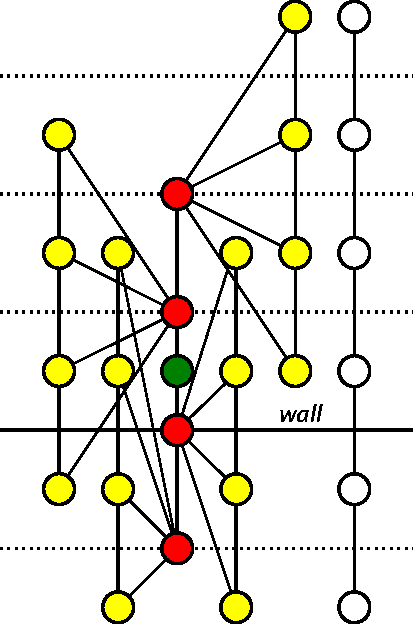
\includegraphics[width=5cm]{figs/stencil_wall.pdf}
		% TO THE TYPESETTER: I have deliberately made this figure smaller in width because it does not need to take up too much space.
	\end{center}
	\caption{Schematic of the diffusion discretization near the wall. The green node is the evaluation point at the center of the first cell above the wall, the red node is the stencil of the divergence operator, and yellow nodes show the stencils of the four gradient operators over which the divergence is evaluated. White nodes indicate the extent of the stencil.} \label{fig:stencil_wall}
\end{figure}
% \begin{eqnarray}
% \nonumber
% \left. \kappa_\phi \dfrac{\partial^2 \phi}{\partial x^2}\right|_{i,j} & = & \kappa_\phi
% \left( \left. \dfrac{\partial \phi}{\partial x}\right|_{i-\frac{3}{2},j} 
% - 27 \left. \dfrac{\partial \phi}{\partial x}\right|_{i-\frac{1}{2},j} \right. \\
% \nonumber
% & & \left. + 27 \left. \dfrac{\partial \phi}{\partial x}\right|_{i+\frac{1}{2},j} 
% - \left. \dfrac{\partial \phi}{\partial x}\right|_{i+\frac{3}{2},j} \right)\\
% & & / \left( x_{i-\frac{3}{2}} - 27    x_{i-\frac{1}{2}} + 27    x_{i+\frac{1}{2}} -    x_{i+\frac{3}{2}} \right)
% \end{eqnarray}
\subsection{Pressure}
Eqs. \ref{eq:presa} and \ref{eq:presb} are solved following the method of \citet{Chorin1968}. This is a fractional step method that first computes intermediate values of the velocity components for the next time step, based on all right hand side terms of the momentum conservation equation Eq. \ref{eq:consmoma}
\begin{eqnarray}
\left. u_i^* \right|^{t+1}_{i,j,k} & = & \left. u_i \right|^{t}_{i,j,k} + \Delta t \left. f_i \right|^{t}_{i,j,k},
\end{eqnarray}
with the intermediate velocity components denoted with an asterix.

The velocity values at the next time step can be computed as soon as the pressure is known, using
\begin{eqnarray}
\left. u_i\right|^{t+1}_{i,j,k} & = & \left. u_i^* \right|^{t+1}_{i,j,k} - \Delta t \left. \delta^{nx_i}\left( \dfrac{p}{\rho_0}\right)\right|^t_{i,j,k}.
\end{eqnarray}
In order to compute the pressure, we multiply the previous equation with the reference density and take its gradient, arriving at
\begin{eqnarray}
\nonumber \left. \delta^{nx_i} \left( \rho_0 u_i\right) \right|^{t+1}_{i,j,k} & = & 
\left. \delta^{nx_i} \left( \rho_0 u_i^* \right) \right|^{t+1}_{i,j,k}\\
& - &  \Delta t \left.\delta^{nx_i} \left[ \rho_0 \delta^{nx_i}\left( \dfrac{p}{\rho_0}\right) \right] \right|^t_{i,j,k},
\end{eqnarray}
where $n$ indicates the spatial order, and the subscript $i$ in superscript $x_i$ indicates that $\delta^{nx_i}$ is a divergence operator. The left hand side equals zero due to mass conservation at the next time step (Eq. \ref{eq:consmassa}). The resulting equation is the Poisson equation that is the discrete equivalent of Eq. \ref{eq:presa}. Rewriting this equation leads to
\begin{eqnarray}
\dfrac{\left. \delta^{nx_i} \left( \rho_0 u_i^* \right) \right|^{t+1}_{i,j,k}}{\Delta t}
& = &  \left. \delta^{nx_i} \left[ \rho_0 \delta^{nx_i}\left( \dfrac{p}{\rho_0}\right) \right] \right|^t_{i,j,k}.
\end{eqnarray}
To simplify the notation, we denote the left-hand side term as $\psi$ and the $p / \rho_0$ term on the right hand side as $\pi$. Solving a Poisson equation is a global operation. Because the computed fields are periodic in the horizontal directions on an equidistant grid, and a Poisson equation is linear, we can perform a Fourier transform in the two horizontal directions
\begin{eqnarray}
\widehat{\psi}_{l,m,k} = - k^2_{*n} \widehat{\pi}_{l,m,k} - l^2_{*n} \widehat{\pi}_{l,m,k}
+ \delta^{nz} \left[ \rho_0 \delta^{nz} \left( \widehat{\pi} \right) \right]_{l,m,k},\label{eq:presfourier}
\end{eqnarray}
where Fourier transformed variables are denoted with a hat, the spatial order of the operation with $n$, and the wave numbers in the two horizontal dimensions $x$ and $y$ are $l$ and $m$ respectively. Variables $k_*^2$ and $l_*^2$ are the squares of the modified wave numbers
\begin{eqnarray}
-k_{*2}^2 & \equiv & 2 \dfrac{\cos (k \Delta x)}{\left( \Delta x \right)^2} - \dfrac{2}{\left( \Delta x \right)^2}
\end{eqnarray}
and
\begin{eqnarray}
\nonumber
-k_{*4}^2 & \equiv & 2 \dfrac{\cos (3k \Delta x) - 54 \cos (2k \Delta x) + 783 \cos (k \Delta x)}
{576 \left( \Delta x \right)^2}\\
& - & \dfrac{1460}{576 \left( \Delta x \right)^2},
\end{eqnarray}
where the former is the modified wave number for the second-order accurate solver and the latter is the wave number for the fourth-order one. Note that the coeffecients correspond to those in Eqs. \ref{eq:diff_2nd} and \ref{eq:diff_4th}. Both expressions satisfy the limit $\lim_{\Delta x \rightarrow 0} k_{*n}^2 = k^2$, where $n$ is the order of the scheme.

Solving Eq. \ref{eq:presfourier} for $\widehat{\pi}$ requires solving a banded matrix for the vertical direction in which the walls are located. This matrix is tridiagonal for the second-order solver and hepta-diagonal for the fourth-order solver. For this, a standard Thomas algorithm \citep{Thomas1949} is used. After the pressure is acquired, inverse Fourier transforms are applied and subsequently the pressure gradient term (see Eqs. \ref{eq:consmoma} and \ref{eq:consmomb}) is computed for all three components of the velocity tendency. Note that the computation of the corrected velocity components does not require a boundary condition for pressure (see \citet{Vreman2014} for details).

\subsection{Thermodynamics}\label{sec:thermo}
MicroHH supports the potential  ($\theta$) and liquid water potential ($\theta_\mathrm{l}$) temperature as thermodynamic variables (Sect. \ref{sec:conservation_of_energy}). The dry ($\theta$) and moist ($\theta_\mathrm{l}$) thermodynamics are related through the use of a total specific humidity $q_\mathrm{t}$, which is defined as the sum of the water vapour specific humidity ($q_\mathrm{v}$) and the cloud liquid water specific humidity ($q_\mathrm{l}$). In the absence of liquid water, $\theta_\mathrm{l} = \theta$, in the presence of liquid water, the liquid water potential temperature is approximated as \citep{Betts1973}

\begin{equation}
\theta_\mathrm{l} \approx \theta - \frac{L_\mathrm{v}}{c_\mathrm{p} ~ \Pi} q_\mathrm{l}, 	
\end{equation}

\noindent where $L_\mathrm{v}$ is the latent heat of vaporization, $c_\mathrm{p}$ the specific heat of dry air at constant pressure, and $\Pi$ is the Exner function

\begin{equation}
\Pi = \left( \frac{p}{p_{00}} \right)^{R_\mathrm{d} / c_\mathrm{p}},
\end{equation}

\noindent where $p$ is the hydrostatic pressure, $p_\mathrm{00}$ a constant reference pressure, and $R_\mathrm{d}$ the gas constant for dry air. The cloud liquid water content is calculated as

\begin{equation}
q_\mathrm{l} = \mathrm{max}(0, ~q_\mathrm{t} - q_\mathrm{s}),
\end{equation}

\noindent where $q_\mathrm{s}$ is the saturation specific humidity

\begin{equation}
q_\mathrm{s} = \frac{\epsilon ~ e_\mathrm{s}}{p - (1-\epsilon) ~ e_\mathrm{s}},
\end{equation}

\noindent with $\epsilon$ the ratio between the gas constant for dry air and the gas constant for water vapour ($R_\mathrm{d}/R_\mathrm{v}$), and $e_\mathrm{s}$ the saturation vapor pressure. The latter is approximated using a 10$^\mathrm{th}$ order Taylor expansion at $T=$ 0 degree Celsius of the Arden Buck equation \citep{Buck1981}. $q_\mathrm{l}$ is adjusted iteratively to arrive at a consistent state where $q_\mathrm{v} = q_\mathrm{s}$. Finally, the virtual potential temperature (Eq. \ref{eq:consmoma}) is defined in MicroHH as 

\begin{equation}
\theta_\mathrm{v} \equiv  \theta \left(1-\left[1-\frac{R_\mathrm{v}}{R_\mathrm{d}}\right] q_\mathrm{t} - \frac{R_\mathrm{v}}{R_\mathrm{d}} q_\mathrm{l} \right)
\end{equation}
The base state pressure and density are calculated assuming a hydrostatic equilibrium: $\mathrm{d}p_0 = -\rho_0 g \mathrm{d}z$, with the density defined as $\rho_0 = p_0 / (R_\mathrm{d} ~ \Pi ~ \theta_\mathrm{v0})$. Integration with height results in

\begin{equation}
p_{0;k+1} = p_{0;k} ~ \mathrm{exp}\left(\frac{-g (z_{k+1}-z_k)}{R_\mathrm{d} ~ \Pi ~ \theta_\mathrm{v0}} \right )
\end{equation}

\noindent where $\theta_\mathrm{v0}$ is the average virtual potential temperature between $z_k$ and $z_{k+1}$. This equation is applied from a given surface pressure to the model top, alternating the calculations at the full and half model levels. That is, given the full thermodynamic state (pressure and density) at a full level $k$, the thermodynamic state can be advanced from the half level $k-\frac{1}{2}$ to $k+\frac{1}{2}$. Using the newly calculated state at $k+\frac{1}{2}$, pressure and density at $k+1$ can be calculated. 

The base state density $\rho_0$ that is used in the dynamical core (Sect. \ref{sec:dyncore}) is calculated using the initial virtual potential temperature profile, and is not updated during the experiment. The density and hydrostatic pressure used in the moist thermodynamics can optionally be updated every time step, following the same procedure as explained in \citet{Boing2014}.

\subsection{Rotation}
The effects of a rotating reference can be included through the Coriolis force. MicroHH can run on an $f$-plane, where the related tendencies of the two horizontal velocity components are calculated as
\begin{eqnarray}
\left. \dfrac{\partial u}{\partial t}\right|_{i,j,k,F_\textrm{cor}} & = & f_0 v_{i,j,k},\\
\left. \dfrac{\partial v}{\partial t}\right|_{i,j,k,F_\textrm{cor}} & = & -f_0 u_{i,j,k},
\end{eqnarray}
with $f_0$ as Coriolis parameter specified by the user.

\section{Physical parameterizations}\label{sec:parametrizations}

\subsection{Subfilter-scale model for large-eddy simulation}
With the governing equations described in Sect. \ref{sec:dyncore} it is possible to resolve the flow down to the scales where molecular viscosity acts. In many applications, however, such simulations are too costly. In that case, one may opt for large-eddy simulation (LES), where filtered equations are used to describe the largest scales of the flow, and the subfilter-scale motions are modeled. The LES implementation in MicroHH assumes very high Reynolds numbers in which the molecular viscosity is neglected. MicroHH uses the grid scale as an implicit filter, rather than applying explicit filtering. Filtering of the anelastic conservation of momentum equation (Eq. \ref{eq:consmoma}), with a tilde applied to denote filtered variables, leads to 
\begin{eqnarray}
\nonumber \dfrac{\partial \uf_i}{\partial t} & = & - \dfrac{1}{\rho_0} \dfrac{\partial \rho_0 \uf_i \uf_j}{\partial x_j} 
- \dfrac{\partial \pi}{\partial x_i} - \dfrac{1}{\rho_0} \dfrac{\partial \rho_0 \tau_{ij}}{\partial x_j}\\
& + & \delta_{i3} g \dfrac{\thetaf_v'}{\theta_{v0}} + F_i.\label{eq:consmoma_filter}
\end{eqnarray}
In this equation, a tensor $\tau_{ij}$ is defined as
\begin{eqnarray}
\tau_{ij}  & \equiv & \widetilde{u_i u_j} - \uf_i \uf_j - \frac{1}{3} \left( \widetilde{u_i u_i} - \uf_i \uf_i \right).
\end{eqnarray}
This is the anisotropic subfilter-scale kinematic momentum flux tensor. The isotropic part of the full momentum flux tensor has been added to the pressure, providing the modified pressure
\begin{eqnarray}
\pi & \equiv & \dfrac{\widetilde{p}^\prime}{\rho_0} + \frac{1}{3} \left( \widetilde{u_i u_i} - \uf_i \uf_i \right).
\end{eqnarray}
As $\tau_{ij}$ contains the filtered product of unfiltered velocity components, this quantity needs to be parameterized. MicroHH uses the Smagorinsky-Lilly \citep{Lilly1968} model, in which $\tau_{ij}$ is modeled as
\begin{eqnarray}
\tau_{ij} & = & -K_m \left( \dfrac{\partial \uf_i}{\partial x_j} + \dfrac{\partial \uf_j}{\partial x_i} \right),
\end{eqnarray}
with $K_m$ interpreted as the subfilter eddy-diffusivity. This quantity is modeled as 
\begin{eqnarray}
K_m    & = & \lambda^2 S
\left(1 - \dfrac{N^2}{Pr_t S^2} \right)^\frac{1}{2},
\end{eqnarray}
and is proportional to the magnitude $S \equiv \left( 2 S_{ij} S_{ij} \right)^\frac{1}{2}$ of the strain tensor $S_{ij}$, which is defined as
\begin{eqnarray}
S_{ij} & \equiv & \frac{1}{2} \left( \dfrac{\partial \uf_i}{\partial x_j} + \dfrac{\partial \uf_j}{\partial x_i} \right).
\end{eqnarray}
The subfilter eddy diffusivity thus takes into account the local stratification $N^2$ and the turbulent Prandtl number $Pr_t$. The latter is set to $\frac{1}{3}$ by default, but can be overridden in the settings. The length scale  $\lambda$ is the mixing length defined following \citet{Mason1992}, as
\begin{eqnarray}
\dfrac{1}{\lambda^n} = \dfrac{1}{\left[ \kappa \left(z + z_0 \right) \right]^n} + \dfrac{1}{\left( c_s \Delta \right)^n},
\end{eqnarray}
which is an arbitrary ($n$ is a free parameter, set to 2 in MicroHH) matching function between the mixing length following wall scaling to the subfilter length scale (filter size) $\Delta \equiv (\Delta x \Delta y \Delta z)^\frac{1}{3}$, related to the grid spacing. In case of a high-Reynolds number atmospheric LES with an unresolved near-wall flow, the vertical gradients of the horizontal velocity components $\partial \uf_{i,j}/\partial z$  in the strain tensor are replaced with the theoretical gradients predicted from Monin-Obukhov similarity theory. Evaluation of these gradients is explained in detail in Section \ref{sec:surface_model}.

The same approach is followed for all scalars, including the thermodynamic variables discussed in Sect. \ref{sec:dyncore_energy}:
\begin{eqnarray}
\dfrac{\partial \phif}{\partial t} & = & - \dfrac{1}{\rho_0} \dfrac{\partial \rho_0 \uf_j \phif}{\partial x_j} - \dfrac{1}{\rho_0} \dfrac{\partial \rho_0 R_{\phi,j}}{\partial x_j} + \widetilde{S}_\phi. \label{eq:consscal_filter}
\end{eqnarray}
The term $R_{\phi,j}$ refers to the subfilter flux of $\phif$ and is defined as
\begin{eqnarray}
R_{\phi,j} = \widetilde{u_j \phi} - \uf_j \phif.
\end{eqnarray}
The subfilter-scale flux is parameterized in terms of the gradient
\begin{eqnarray}
R_{\phi,j} = - \dfrac{K_m}{Pr_t} \dfrac{\partial \phif}{\partial x_j}.
\end{eqnarray}

\subsection{Surface model}\label{sec:surface_model}
The LES implementation of MicroHH uses a surface model that is constrained to rough surfaces and high Reynold numbers, which is a typical configuration for atmospheric flows. This model computes the surface fluxes of the horizontal momentum components and the scalars (including thermodynamic variables) using Monin-Obukhov Similarity Theory (MOST) (\citet[][his Sect. 10.2]{Wyngaard2010}). MOST relates surface fluxes of variables to their near-surface gradients using empirical functions that depend on the height of the first model level $z_1$ divided by the Obukhov length $L$ as an argument. Length $L$ is defined as
\begin{eqnarray}
L   & \equiv & - \dfrac{u_*^3}{\kappa B_0},
\end{eqnarray}
where $u_*$ is the friction velocity, $\kappa$ is the Von Karman constant and $B_0$ is the surface kinematic buoyancy flux. $L$ represents the height at which the buoyancy production/destruction of turbulence kinetic energy equals the shear production. In MicroHH, we use a local implementation of MOST, i.e., each grid point has its own value of $L$. This choice can lead to a overestimation of near-surface wind due to violation of the MOST assumption of horizontal homogeneity \citep[][their Fig. 18]{Bouzeid2005}, but it allows for a more straightforward extension to heterogeneous land surfaces.

Following MOST, the friction velocity $u_*$ and the momentum fluxes may be related to the near-surface wind gradient as
\begin{eqnarray}
\dfrac{\kappa z_1}{u_*} \dfrac{\partial U}{\partial z}  \approx 
- \dfrac{\kappa z_1 u_*}{\overline{u^\prime w^\prime}} \dfrac{\partial \uf}{\partial z} \approx
- \dfrac{\kappa z_1 u_*}{\overline{v^\prime w^\prime}} \dfrac{\partial \vf}{\partial z} \approx
\phi_m \left( \dfrac{z_1}{L} \right),\label{eq:surf_grad}
\end{eqnarray}
where $U$ is defined as $\sqrt{\uf^2 + \vf^2}$, and $\overline{u^\prime w^\prime}$ and $\overline{v^\prime w^\prime}$ as the surface momentum fluxes for the two wind components. These relationships can be integrated from the roughness length $z_{0m}$ to $z_1$ resulting in 
\begin{eqnarray}
u_* & =  & f_m \left( U_1 - U_0 \right),\\
\overline{u^\prime w^\prime} & = & - u_* f_m \left( \uf_1 - \uf_0 \right),\\
\overline{v^\prime w^\prime} & = & - u_* f_m \left( \vf_1 - \vf_0 \right),
\end{eqnarray}
with $f_m$ defined as:
\begin{eqnarray}
f_m & \equiv & \dfrac{\kappa}
{ \ln{\left( \dfrac{z_1}{z_{0m}} \right)}
	- \varPsi_m \left( \dfrac{z_1}{L} \right)
	+ \varPsi_m \left( \dfrac{z_{0m}}{L} \right) }, \label{eq:fm}
\end{eqnarray}
with $\varPsi_m$ desribed in Eqs. \ref{eq:psiu} and \ref{eq:psis}.

The same procedure for scalars is followed, with
\begin{eqnarray}
\dfrac{\kappa z_1 u_*}{\overline{\phi^\prime w^\prime}} \dfrac{\partial \phif}{\partial z} =
\phi_h \left( \dfrac{z_1}{L} \right),
\end{eqnarray}
and in integrated form
\begin{eqnarray}
\overline{\phi^\prime w^\prime} & = & u_* f_h \left( \phif_1 - \phif_0 \right),
\end{eqnarray}
with
\begin{eqnarray}
f_h & \equiv &
\dfrac{\kappa}
{ \ln{\left( \dfrac{z_1}{z_{0h}} \right)}
	- \varPsi_h \left( \dfrac{z_1}{L} \right)
	+ \varPsi_h \left( \dfrac{z_{0h}}{L} \right) }, \label{eq:fh}
\end{eqnarray}
with $\varPsi_h$ desribed in Eqs. \ref{eq:psiu} and \ref{eq:psis}.

The functions $\phi_m$, $\phi_h$, $\varPsi_m$, and $\varPsi_h$ are empirical and depend on the static stability of the atmosphere. Under unstable conditions we follow \citep{Wilson2001, Wyngaard2010} 
\begin{eqnarray}
\phi_{m,h} & = & \left( 1 + \gamma_{m,h} \left| \zeta \right|^{2/3} \right)^{-1/2},\label{eq:phiu}\\
%\phi_h & = & \left( 1 + \gamma_h \left| \zeta \right|^{2/3} \right)^{-1/2}\\
\varPsi_{m,h} & = & 3 \ln{\left( \dfrac{1 + \phi_{m,h}^{-1}}{2} \right)},\label{eq:psiu} 
%\Psi_m & = & \left( 1 + (3.6 \frac{z}{L})^{2/3} \right)^{-\frac{1}{2}} \\
%\Psi_h & = & \left( 1 + (3.6 \frac{z}{L})^{2/3} \right)^{-\frac{1}{2}} \\
\end{eqnarray}
where $\zeta$ is the ratio of a height and the Obukhov length $L$, $\gamma_m = 3.6$ and $\gamma_h = 7.9$. Under stable conditions we use \citep{Hogstrom1988, Wyngaard2010}
\begin{eqnarray}
\phi_{m,h} & = & 1 + \lambda_{m,h} \zeta, \label{eq:phis}\\
\varPsi_{m,h} & = & - \lambda_{m,h} \zeta, \label{eq:psis}
\end{eqnarray}
where $\lambda_m = 4.8$ and $\lambda_h = 7.8$.

With the equations above, the surface fluxes, surface values and near-surface gradients can be computed, but only if the Obukhov length $L$ is known. The surface model calculates the Obukhov length by relating the dimensionless parameter $z_1/ L$ to a Richardson number. The employed formulation of the Richardson number depends on the chosen boundary condition in the model. Three possible options are available:
\begin{itemize}
	\item fixed momentum fluxes and a fixed surface buoyancy flux. Both the friction velocity $u_*$ and the surface buoyancy flux $B_0$ are specified. Under these conditions we define the Richardson number $Ri_a$ equal to $z_1/L$; $L$ can be computed directly from the expression
	\begin{equation}
	Ri_a \equiv \dfrac{z_1}{L} = - \dfrac{\kappa z_1 B_0}{u_*^3}.
	\end{equation}
	\item a fixed horizontal velocity $U_0$ at the surface and a fixed surface buoyancy flux $B_0$. The friction velocity $u_*$ is unknown. Now,  $L$ needs to be retrieved from the implicit relationship 
	\begin{equation}
	Ri_b \equiv \dfrac{z_1}{L} f_m^3 = - \dfrac{\kappa z_1 B_0}{ \left(U_1 - U_0 \right)^3}.
	\end{equation}
	\item a fixed surface velocity $U_0$ and a fixed surface buoyancy $b_0$. With this boundary condition, the surface values of the horizontal velocities and the buoyancy are given, and both $u_*$ and the surface buoyancy flux $B_0$ are unknown. $L$ is then retrieved from
	\begin{equation}
	Ri_c \equiv \dfrac{z_1}{L} \dfrac{f_m^2}{f_h} = \dfrac{\kappa z_1 \left(\widetilde{b}_1 - \widetilde{b}_0 \right)}{ \left(U_1 - U_0 \right)^2}.
	\end{equation}
\end{itemize}
In cases of the latter two options, a solver is required to find the $L$ that satisfies the equation, as $f_m$ (Eq. \ref{eq:fm}) and $f_h$ (Eq.  \ref{eq:fh}) both depend on $L$ as well. For performance reasons, we have created a lookup table-based approach that relates $L$ to the Richardson number. The lookup table has $10^4$ entries, of which 90 percent is spaced uniformly between $z_1/L = -5$ to $5$. The remaining 10 percent are used to stretch the negative range up to $z_1/L = -10^4$ to allow for the correct free convection limit. 

\subsection{Large-scale forcings}
\subsubsection{Pressure force}
MicroHH provides two options to introduce a large-scale pressure force into the model. The first is to enforce a constant massflux through the domain in the streamwise direction. In this approach the desired large-scale velocity $U_f$ is set, and the corresponding pressure gradient is computed. We follow here the approach of  \citet{vanReeuwijk2007}. In this approach, the $u$-component of the horizontal momentum equation (Eq. \ref{eq:consmoma}) is volume-averaged to acquire
\begin{eqnarray}
\dfrac{\left< u \right>^{n+1}  - \left< u \right>^{n}}{\Delta t} & = & \left< f_1 
\right> - \left< \dfrac{\partial}{\partial x} \left( \dfrac{p}{\rho_0} \right) \right>
+ F_{p;ls}
\end{eqnarray}
where brackets indicate a volume average, $f_1$ contains all the righthand side terms of the $u$-component of the conservation of momentum, except for the dynamic pressure, which is contained in the second term. The large-scale pressure force $F_{p;ls}$, which is to be computed, is the last term. We can now set $\left< u \right>^{n+1} = U_f$ to explicitly set the volume-averaged velocity in the next time step. Furthermore, the volume-averaged horizontal pressure gradient vanishes, because of the periodic boundary condition, which makes $F_{p;ls}$ the only unknown. The acquired pressure force $F_{p;ls}$ will be added as an external force in the equation of zonal velocity ($F_1$ in Eqs \ref{eq:consmoma} and \ref{eq:consmomb}).

The second option is to enforce a large-scale pressure force through the geostrophic wind components $u_g$ and $v_g$, in combination with rotation, with the tendencies of the two horizontal velocity components calculated as
\begin{eqnarray}
F_{p;ls,1} & = & -f_0 v_{g;k},\\
F_{p;ls,2} & = &  f_0 u_{g;k},
\end{eqnarray}
where $u_{g;k}$ and $v_{g;k}$ as user-specified vertical profiles of geostrophic wind components.

\subsubsection{Large-scale sources and sinks}
Large-scale sources and sinks, representing for instance large-scale advection or radiative cooling, can be prescribed for each variable separately. The user has to provide vertical profiles of large-scale tendencies $S_{\phi;ls}$ that are added to the total tendencies.

\subsubsection{Large-scale vertical velocity}
A second method of introducing large-scale thermodynamic effects is through the inclusion of a large-scale vertical velocity. In this case, each scalar gets an additional tendency term of the form
\begin{eqnarray}
\left. \dfrac{\partial \phi}{\partial t}\right|_{i,j,k,ls} & = &  - w_{ls;k}\,\delta^{2x} \left( \left< \phi \right>_k \right),
\end{eqnarray}
where $\left< \phi \right>_k$ is the horizontally-averaged vertical profile at height $z_k$ for scalar $\phi$. The tendency term is not applied to the momentum variables.

\subsection{Buffer layer}
MicroHH has the option to damp gravity waves in the top of the simulation domain in a so-called buffer layer.  The tendency associated with the damping at grid cell $i,j,k$ is calculated for an arbitrary variable $\phi$ as
\begin{eqnarray}
\left. \dfrac{\partial \phi}{\partial t}\right|_{i,j,k,\textrm{buf}} = \dfrac{\phi_{i,j,k} - \phi_{0;k}}{\tau_{d;k}}
\end{eqnarray}
where $\phi_0$ is taken from a user-specified reference profile, and time scale $\tau_d$ is a measure for the strength of the damping. It varies with height and is calculated at height $z_k$ following
\begin{eqnarray}
\tau_{d;k}^{-1} = \sigma \left( \dfrac{z_k - z_{b;bot} }{z_{b;top} - z_{b;bot}} \right)^\beta,
\end{eqnarray}
where $\sigma$ is the damping frequency chosen by the user and $\beta$ an exponent that describes the shape of the vertical profile of the damping frequency, which is always zero at the bottom ($z_{b;bot}$) and $\sigma$ at the top ($z_{b;top}$)  of the layer.

\section{Technical details of the code}\label{sec:technical}
\subsection{Code structure}
MicroHH is written in C++ and uses elements of object-oriented programming and template metaprogramming. The code components are written in classes that define the interface. Inheritance is used to allow for specializations of classes. This way of organizing the code has two advantages: it minimizes switches and it allows code components and their extensions to reside in their own file, which increases code clarity and facilitates the merging of new code extensions. High performance of computational kernels is achieved by executing kernels in their own function, with explicit inclusions of the \texttt{restrict} keyword to notify the compiler that fields do not overlap in memory. Furthermore, compiler-specific pragmas are used to aid vectorization on Intel compilers.

\subsection{GPU}
MicroHH is enabled to run on fast and energy-efficient Graphical Processing Units (GPU). This promising technique has been pioneered in atmospheric flows by \citet{Schalkwijk2012} and has shown its potential in weather forecasting \citep{Schalkwijk2015}. The implementation is based on NVIDIA's CUDA. The CPU and GPU version reside in the same code base, where the GPU implementation is activated with the help of precompiler statements. The philosophy is that the entire model is initialized on the CPU and that the GPU implementation is only activated right before starting the main time loop.  At that moment, the required fields are copied in double precision accuracy to the GPU, and the entire time integration is done there. Synchronization only happens when statistics have to be computed or when restart files or cross sections of flow fields are saved to disk, to ensure high performance. The design choice to do the entire initialization on the GPU minimizes the amount of GPU code, and therefore allows for maintaining a single code base for the CPU and GPU code.

\subsection{Parallelization}
The code uses the Message Passing Interface (MPI) in order to run on a large number of cores. The three-dimensional simulation domain is split into vertically-oriented columns standing on a two-dimensional grid. The code assigns one MPI task to each grid column using the MPI\_Cart\_create function, and uses this grid to detect the IDs of neighboring processes. In order to avoid complex packing routines, we make use of MPI datatypes wherever possible. The MPI calls are hidden in an interface to avoid the need to manually write MPI calls.

The input/output (IO) is entirely based on MPI-IO, the parallel writing framework that comes with MPI, to ensure that three-dimensional fields and two-dimensional cross sections are stored as single files. We have chosen MPI-IO in order to limit the number of files resulting from simulations on a large number of processes and to allow for restarts on a different number of processes. In order to keep complexity of the IO as low as possible, we make use of the MPI\_Sub\_array function in combination with MPI\_File\_write\_all in order to write the fields.

\subsection{External dependencies}
MicroHH depends on several external software tools or libraries. It uses the CMake (\url{https://cmake.org}) build system for the generation of Makefiles. CMake allows for parallel builds, which minimizes the compilation time, and it is easy to add configurations for different machines. Furthermore, the FFTW3 library \citep{Frigo2005} is used for the computation of fast-Fourier transforms. The statistical routines make use of netCDF software developed by UCAR/Unidata (\url{http://doi.org/10.5065/D6H70CW6}). In order to run the provided test cases and their output scripts, a Python (\url{https://www.python.org}) installation including the NumPy (\url{http://www.numpy.org}) and Matplotlib (\url{https://matplotlib.org}) modules is required. Automatic documentation generation can be done using Doxygen (\url{http://doxygen.org}), but this is optional.

\section{Running simulations}\label{sec:running}
\label{sec:running_simulations}
In order to run a simulation with MicroHH, a sequence of steps needs to be taken. Each simulation has an \texttt{.ini} file that contains the settings of the simulation, a \texttt{.prof} file that contains the (initial) vertical profiles of all required variables, and, if time-varying boundary conditions are desired, a file with the prescribed time evolution for all time-varying boundary conditions. MicroHH provides a document (\texttt{doc/input.pdf}) that contains an overview of all possible options that can be specified in the \texttt{.ini} file.

To prepare a simulation with the name \texttt{test\_simulation}, MicroHH needs to be run in the following way
\begin{verbatim}
./microhh init test_simulation
\end{verbatim}
where it is assumed that \texttt{test\_simulation.ini} and \texttt{test\_simulation.prof} are available in the directory where the command is triggered. This procedure will create the initial fields of all prognostic variables and save the required fields for those model components that need to save their state to guarantee bitwise identical restarts. 

After the previously described initialization phase, the execution of
\begin{verbatim}
./microhh run test_simulation
\end{verbatim}
will start the actual simulation. Depending on the chosen output intervals, the simulation will create restart files, statistics, cross sections, and field dumps. MicroHH can restart from any time at which the restart files are saved.

The last mode in which the code can run is the post-processing mode. By running 
\begin{verbatim}
./microhh post test_simulation
\end{verbatim}
the code will generate statistics from saved restart files at a specified time interval. This mode allows the user to create new statistics and calculate those from saved data, without having to rerun the simulation.

\section{Model output}\label{sec:output}
\subsection{Statistics}
A large set of output statistics can be computed during runtime at user-specified time intervals. The statistics module provides vertical profiles of means, second-, third- and fourth-order moments of all prognostic variables, as well as advective and diffusive fluxes. Furthermore, there are multiple diagnostic variables, such as the pressure, the pressure variance and its vertical flux. The thermodynamics generate their own statistics based on the chosen option. The moist thermodynamics provides a large set of cloud statistics.

There is a separate module for budget statistics, which provides the budgets of all components of the Reynolds stress tensor, and those of the variance and vertical flux of the thermodynamic variables.

One of the key features of the MicroHH statistics routine is that an arbitrary mask can be passed into the routine over which the statistics are calculated. This allows, for instance, for a very simple way of computing conditional statistics in updrafts or clouds, which is demonstrated later in Section \ref{sec:bomex}.

\subsection{Two- and three-dimensional output}
It is possible to save two-dimensional cross sections and three-dimensional fields of any of the prognostic and diagnostic variables of the model, as well as of derived variables. This output can be made at user-specified time intervals. Cross sections can be made in any chosen $xy-$, $xz-$, and $yz-$plane. Derived variables (any arbitrary function of existing model variables), can be easily added to the code by the user.


 \section{Validation of the dynamical core} \label{sec:tests}
In this section, we present a series of cases intended to validate MicroHH under a wide range of settings. Each of these test cases is available in the \texttt{cases/} directory in the MicroHH repository, where all detailed settings can be found (see Sect. \ref{sec:howto}). Below, we present only the most relevant information per case.

\subsection{Taylor-Green vortex}
The two-dimensional Taylor-Green vortex (\texttt{cases/taylorgreen}) presents an ideal test case for a dynamical core as it has an analytical solution, even though it is nonlinear. This flow is composed of two rotating vortices whose evolution in a domain $\left[0,1; 0,0.5 \right]$ is described with
\begin{eqnarray}
u(x,z,t) & = & \sin(2\pi x) \cos(\pi z) f(t),\\
w(x,z,t) & = & \cos(2\pi x) \sin(\pi z) f(t),\\
p(x,z,t) & = & \tfrac{1}{4} \left(\sin(4 \pi x) + \sin(4 \pi z) \right) f(t)^2,
\end{eqnarray}
where $f(t) = 8 \pi^2 \nu t$.

We use the analytical form at $t=0$ as the initial condition and run this case for one vortex rotation ($t = 1$), with $\nu = (800 \pi^2)^{-1}$. We compare the result against the analytical solution for a set of grid spacings and with the second-order and fourth-order dynamical core; for the latter we compare the most accurate advection scheme and the fully energy-conserving one.
\begin{figure}[t]
	\vspace*{2mm}
	\begin{center}
		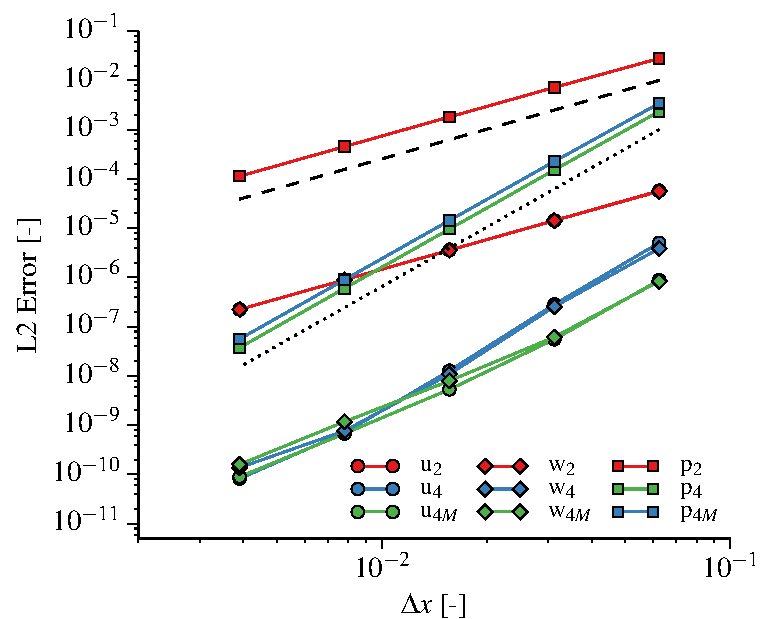
\includegraphics[width=8.3cm]{figs/taylorgreen.pdf}
	\end{center}
	\caption{Convergence of the spatial discretization error in the two-dimensional Taylor-Green vortex. Subscript $2$ indicates the second-order scheme, $4$ the most accurate fourth-order scheme, and $4M$ the fully energy-conserving fourth-order scheme. The dashed black line is the reference for second-order convergence, the dotted black lines indicate fourth-order convergence.}\label{fig:taylorgreen}
\end{figure}

Figure \ref{fig:taylorgreen} shows the error convergence of the simulations. The error for a variable $\phi$ is computed as $\sum \Delta x \Delta z \left| \phi_{i,k} - \phi_{\textrm{ref},i,k}, \right|$ over the two-dimensional domain, where $\Delta x$ and $\Delta z$ are the uniform grid spacings used in this case and $\phi_{\textrm{ref}}$ is the analytical solution. All variables converge according to the order of the numerical scheme. The fourth-order dynamical core loses accuracy at fine grid spacings. This is due to the boundary condition for the vertical velocity that sacrifies an order of accuracy to ensure global mass conservation \citep{Morinishi1998}.

\subsection{Kinetic energy conservation and time accuracy} \label{sec:validationtime}
The second test of the dynamical core consists of combined evaluation of kinetic energy ($u^2 + v^2 + w^2$) conservation and time accuracy 
(\texttt{cases/conservation}). In this experiment, we run the model with only the advection and pressure solver enabled and advect random noise through the domain for 1000 seconds. These tests have been conducted with the third- and fourth-order Runge-Kutta schemes. We have chosen the fourth-order spatial discretization in order to demonstrate its energy conservation.
\begin{figure}[t]
\vspace*{2mm}
\begin{center}
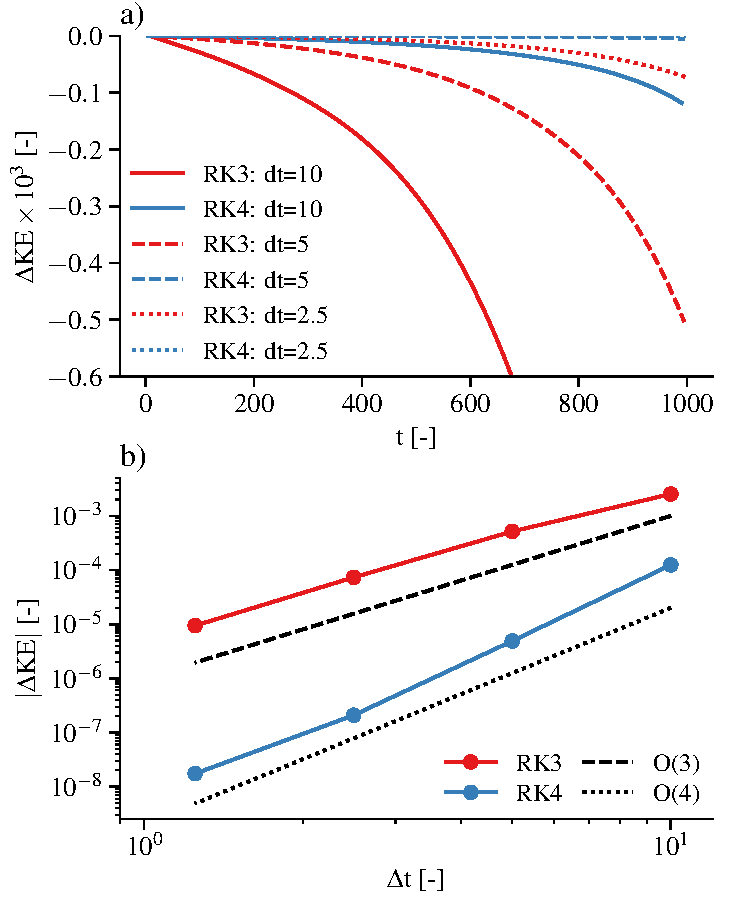
\includegraphics[width=8.3cm]{figs/timeconvergence.pdf}
\end{center}
\caption{Time evolution of the energy loss during 1000 time units of random noise advection for the RK3 and RK4 time integration schemes with three different time steps (a). Error convergence of the temporal discretization for the RK3 and RK4 scheme (b).}\label{fig:timeconvergence}
\end{figure}

The loss of kinetic energy as a function of time is shown in Fig. \ref{fig:timeconvergence}a. The fourth-order scheme results in a smaller energy loss for the same time step and an a faster convergence. The error-convergence plot (Fig. \ref{fig:timeconvergence}b) shows that the error convergence is in accordance with the order of the respective scheme. Furthermore, it illustrates the fact that, if high accuracy in time is desired, the five-stage fourth-order scheme is less expensive than the three-stage third-order scheme. For instance, at a $\Delta t$ of 10, the error of the fourth-order scheme is approximately equal to the error of the third-order scheme at a $\Delta t$ of 2.5. To reach this accuracy, the fourth-order scheme needs only 5 steps per 10 time units, whereas the third-order scheme needs 12 steps.

\subsection{Laminar anabatic flow} \label{sec:laminaranabatic}
To test the buoyancy routine and the option to put the domain on a slope, a Prandl-type anabatic slope flow  \citep{Prandtl1942} has been simulated (\texttt{cases/prandtlslope}). In this test case, the surface is inclined at an angle of $30^{\circ}$ and a linearly stratified atmosphere ($N = 1$~s$^{-1}$) is heated from below with a fixed surface buoyancy flux of 0.05~m$^2$~s$^{-3}$.

\begin{figure}[t]
	\vspace*{2mm}
	\begin{center}
		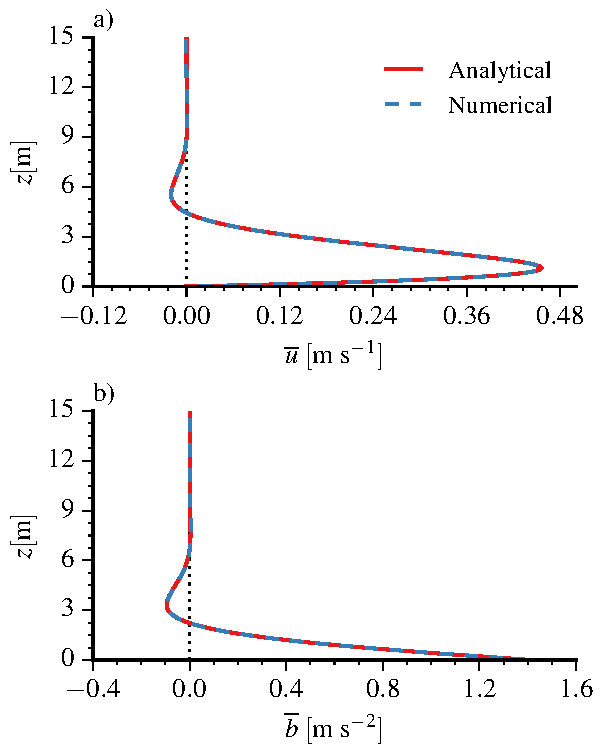
\includegraphics[width=8.3cm]{figs/prandtlslope.pdf}
	\end{center}
	\caption{Normalized numerical Prandtl-model solutions for velocity $u$ (left) and buoyancy $b$ (right) compared to their analytical counterparts.}
	\label{fig:prandtl}
\end{figure}

The fluid, which was initially at rest, goes through a series of decaying oscillations after the  buoyancy flux is applied at the surface. Eventually, it reaches the steady state corresponding to the Prandtl model solution. Numerical integration was performed sufficiently long for the oscillation amplitude to become a small fraction of the amplitude of the first oscillation. Comparison of horizontal wind $u$ and buoyancy $b$ of analytical and numerical solutions is shown in Fig.~\ref{fig:prandtl}. For both variables the solutions closely agree with each other.

\subsection{Turbulent channel flow}
For fully turbulent flows, the numerical solutions cannot be compared against any analytical testcases. Therefore, we validate our results against a channel flow at a Reynolds-$\tau$  number of 590 \citep{Moser1999} for means, variances, spectra, and second-order budget statistics (\texttt{cases/moser590}). The case is run at a resolution of 768 $\times$ 384 $\times$ 256 grid points. The original numerical simulation data of \citet{Moser1999} has been produced on a 384 $\times$ 384 $\times$ 256 grid, with spectral schemes in the horizontal dimensions and Chebyshev polynomials in the vertical.
\begin{figure}[t]
	\vspace*{2mm}
	\begin{center}
		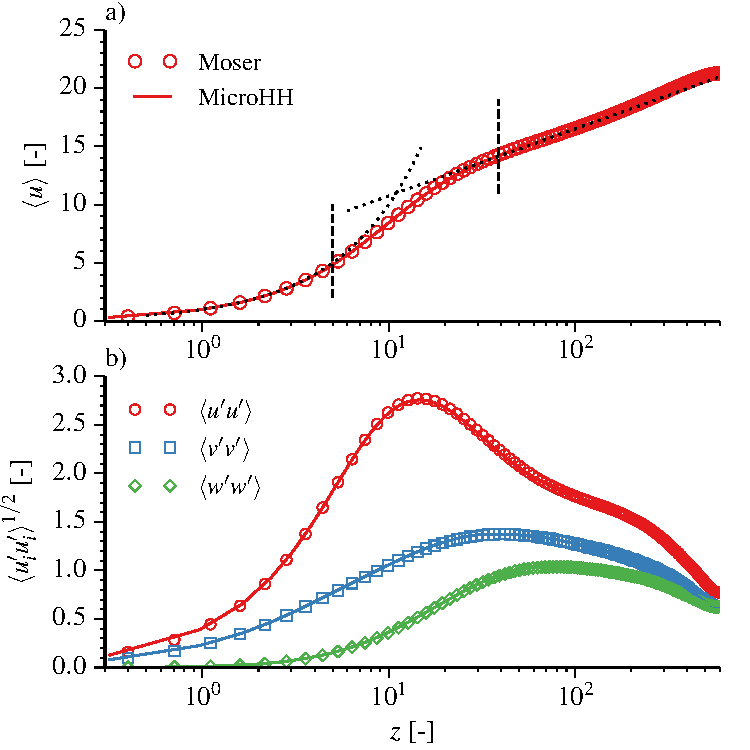
\includegraphics[width=8.3cm]{figs/gmd_m590_umean_var.pdf}
	\end{center}
	\caption{Velocity means and variances for \citet{Moser1999} channel flow case at Reynolds-$\tau$ 590. The dashed vertical lines marks the spectra locations. Height $z$ is normalized with $u_\tau / \nu$, velocities with $u_\tau^{-1}$.}\label{fig:moser_velocity}
\end{figure}

Figure \ref{fig:moser_velocity}a shows the normalized horizontally-averaged streamwise velocity. The normalized rms of all three velocity components are presented in Fig. \ref{fig:moser_velocity}b. All plotted variables show a perfect match with the data and are indistinguishable from Moser's data. In order to further assess the accuracy of the data, we show the second-order budgets of the variances in Fig. \ref{fig:moser_budget}. Also here, the match with the reference data is excellent, which indicates that the whole range of spatial scales in the flow is represented well and that the fourth-order scheme is well able to pick up the small-scale details of the flow.

The findings in the previous paragraph are further corroborated by the spectra shown in Fig. \ref{fig:moser_spectra}.  Over the whole range of scales, the match between our simulation and that of \citet{Moser1999} is excellent. Note that the spectra from Moser's simulation display an increase in pressure variance at the highest wave numbers. This increase is the result of aliasing errors at high wave numbers that are typical for the spectral schemes that \citet{Moser1999} used.

%% TWO-COLUMN FIGURES
\begin{figure*}[t]
\vspace*{2mm}
\begin{center}
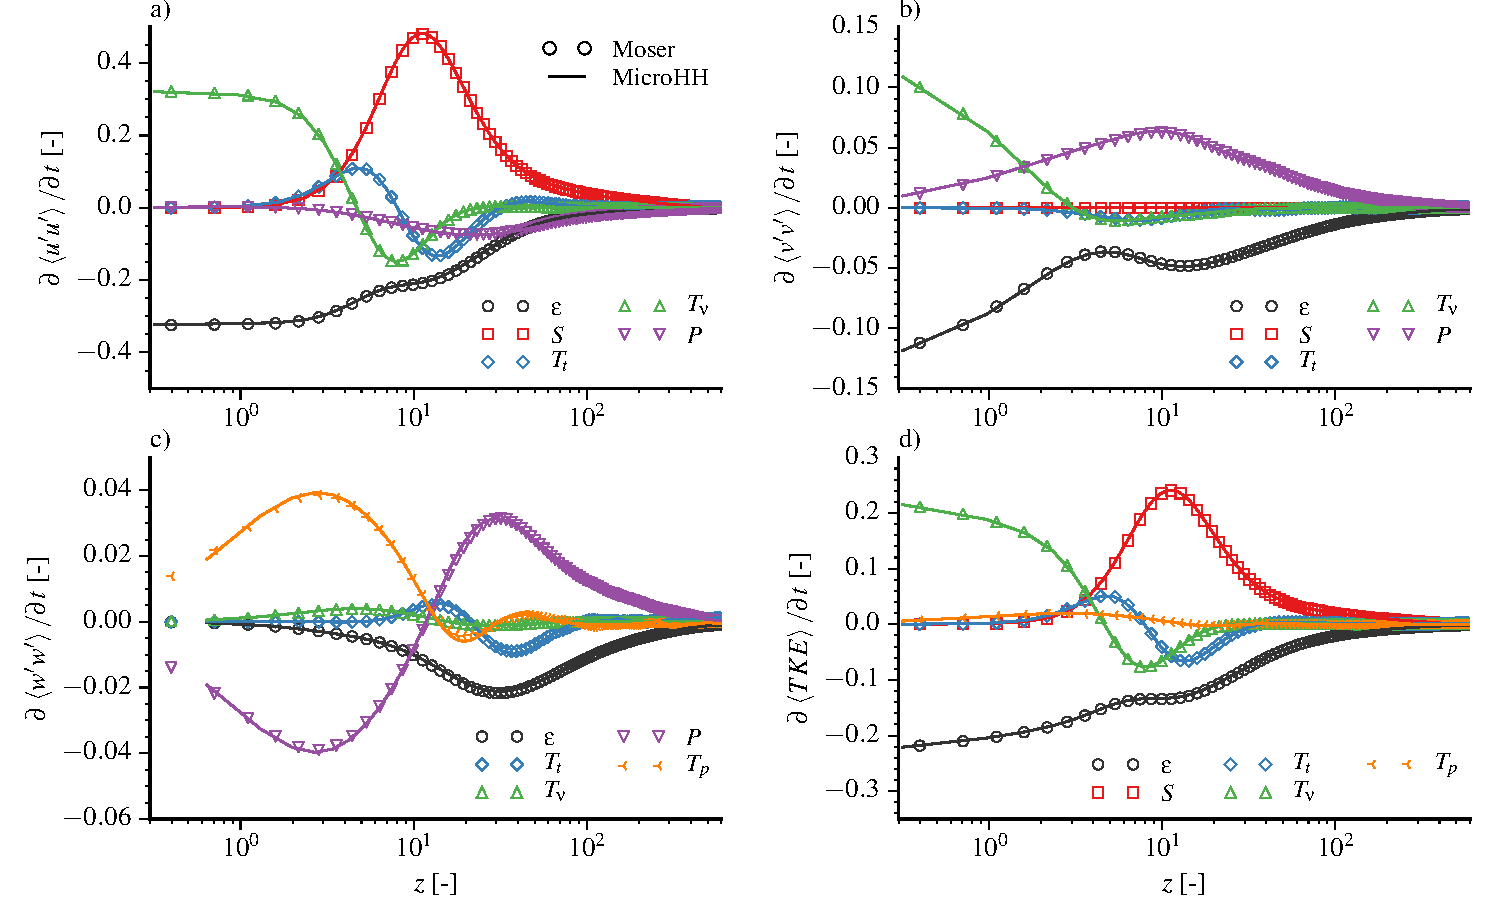
\includegraphics[width=16.6cm]{figs/gmd_m590_turb_budg.pdf}
\end{center}
\caption{Budgets of variances and TKE compared against \citet{Moser1999}'s reference data at Reynolds-$\tau$ of 590. Height $z$ is normalized with $u_\tau / \nu$, the variances and TKE budget with $\nu / u_\tau^{4}$.}\label{fig:moser_budget}
\end{figure*}

%% TWO-COLUMN FIGURES
\begin{figure*}[t]
\vspace*{2mm}
\begin{center}
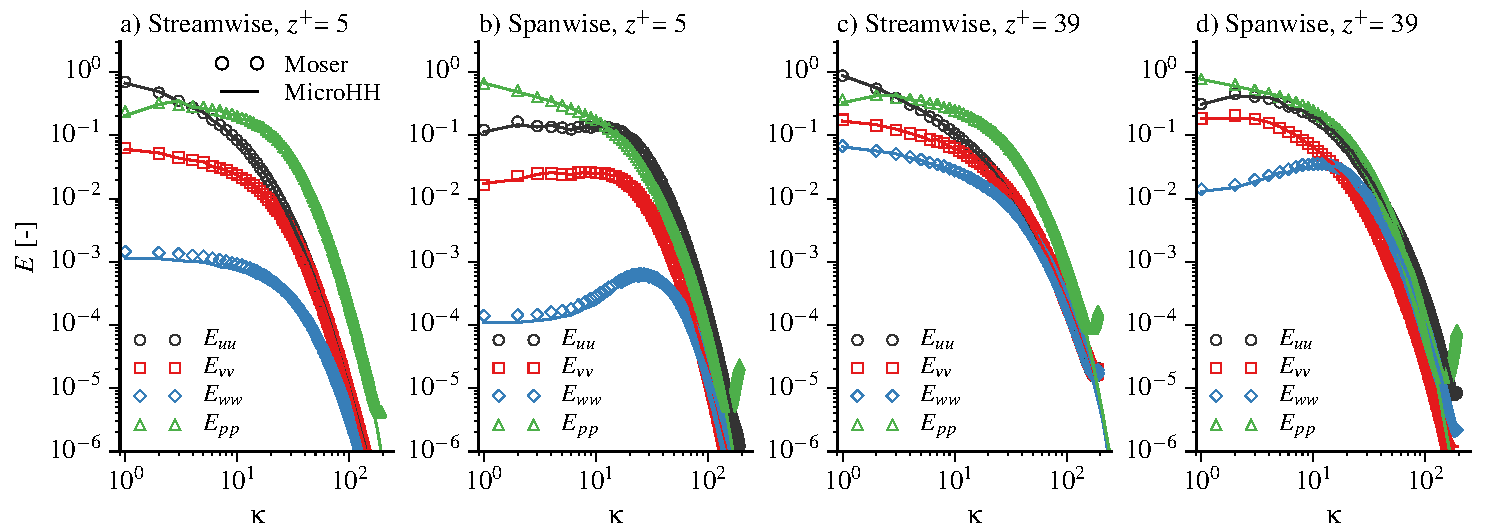
\includegraphics[width=16.6cm]{figs/gmd_m590_spectra_4x1.pdf}
\end{center}
\caption{Spectra of all velocity components and pressure compared against \citet{Moser1999}'s reference data at Reynolds-$\tau$ of 590. The velocity spectra are normalized with $u_\tau^{-2}$, the pressure spectra with $u_\tau^{-4}$}\label{fig:moser_spectra}
\end{figure*}

\subsection{Turbulent katabatic flow}
The final evaluation of the dynamical core without parametrizations enabled is based on the direct numerical simulation of a turbulent katabatic flow. Here, a buoyancy driven slope flow is simulated following the setup of \citet{Fedorovich2009} (\texttt{cases/drycblslope}). A flow over a slope inclined at an angle $\alpha$ of 60$^\circ$ is simulated with a fixed uniform surface buoyancy flux of -0.5~m$^2$~s$^{-3}$. The simulation is performed in a domain of 0.64 m $\times$ 0.64 m $\times$ 1.6 m using a uniform grid of 256 $\times$ 256 $\times$ 640 points. The initial state is a fluid at rest with a linear buoyancy stratification $N$ of 1~s$^{-1}$. No-slip boundary conditions are applied at the bottom, free-slip at the top.

Turbulent motion starts quickly after the buoyancy flux is applied at the surface. It is characterized by random, large-amplitude fluctuations of velocity and buoyancy fields in the near-slope core region, and shows a quasi-periodic oscillatory behavior at larger distances from the slope. Mean profiles of along-slope velocity component and buoyancy, as well as profiles of second-order turbulence statistics, such as kinematic turbulent fluxes of momentum and buoyancy, and velocity-component and buoyancy fluctuation variances, were evaluated by averaging the simulated flow fields spatially over the along-slope planes and temporally over five oscillation periods beyond the transition stage.

For comparison, the same katabatic flow case was reproduced using the numerical code (hereafter referred to as FS09) that was employed to simulate turbulent slope flows in \citet{Shapiro2008} and \citet{Fedorovich2009}. In that code, the time advancement was performed with an Asselin-filtered second-order leapfrog scheme \citep{Durran2013}. The spatial discretizations are identical to the second-order accurate ones of MicroHH. 

Numerical results obtained with both numerical codes testify that stable environmental stratification in combination with negative surface buoyancy forcing in the katabatic flow leads to an effective suppression of vertical turbulent exchange in the flow region adjacent to the slope. This suppression results in a shallow near-surface sublayer with strong buoyancy gradients (Fig.~\ref{fig:katabatic}a) capped by a narrow jet with peak velocity located very close to the ground (Fig.~\ref{fig:katabatic}b). Further comparison has been performed on the slope-normal fluxes of momenum and buoyancy (not shown), where a nearly perfect match has been reproduced as well.

\begin{figure}[t]
	\vspace*{2mm}
	\begin{center}
		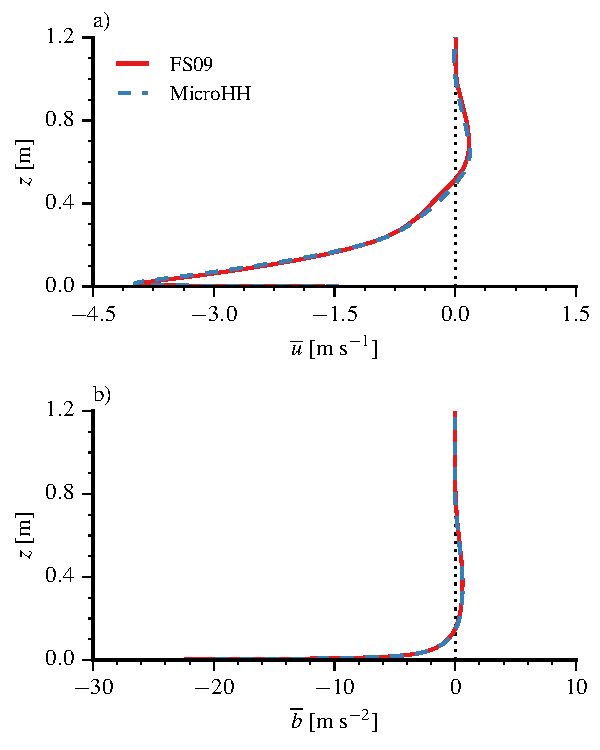
\includegraphics[width=8.3cm]{figs/katabatic.pdf}
	\end{center}
	\caption{Profile of the mean along-slope velocity (a) and buoyancy (b) as predicted by MicroHH and FS09.}
	\label{fig:katabatic}
\end{figure}

\section{Validation of atmospheric large-eddy simulations}\label{sec:validation_atmos}
\subsection{Dry convective boundary layer with strong inversion}
As a first test case of MicroHH in LES mode, we present that of \citet{Sullivan2011} (\texttt{cases/sullivan2011}). This is a dry clear convective boundary layer that grows into a linearly stratified atmosphere with a very strong capping inversion (see Fig. \ref{fig:sullivan2011}a). The system is heated from the bottom by applying a constant kinematic heat flux of 0.24~K~m~s$^{-1}$. The domain size is 5120~m $\times$ 5120~m $\times$ 2048~m. Gravity wave damping has been applied in the top 25 percent of the domain. Simulations have been run for three hours with three spatial resolutions. The time-averaged profiles have been calculated over the last hour.

\begin{figure}[t]
	\vspace*{2mm}
	\begin{center}
		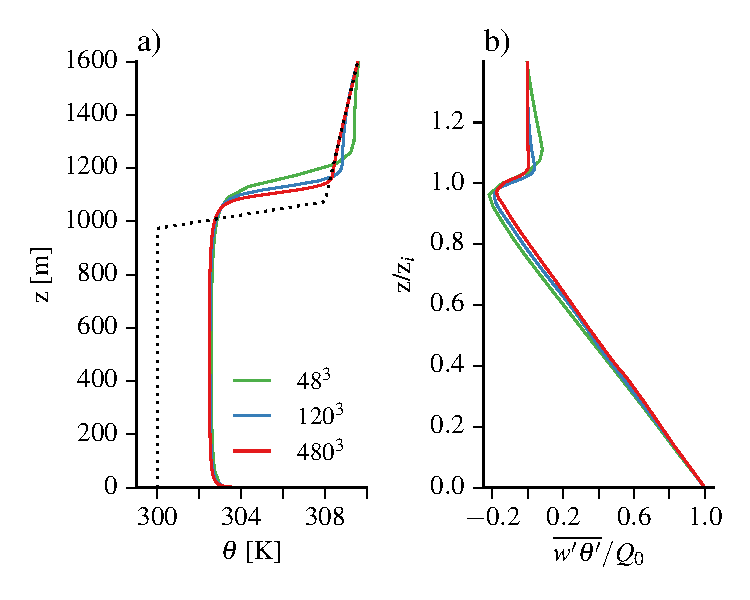
\includegraphics[width=8.3cm]{figs/sullivan2011.pdf}
	\end{center}
	\caption{Vertical profiles of horizontally-averaged potential temperature (a) and normalized kinematic heat flux (b). The boundary layer depth $z_i$ is the location of the maximum vertical gradient in the potential temperature profile shown in (a). }
	\label{fig:sullivan2011}
\end{figure}

The results show the formation of a well-mixed layer with an overlying capping inversion (see Fig. \ref{fig:sullivan2011}a) and the associated linear heat-flux profile with negative flux values in the entrainment zone (see Fig. \ref{fig:sullivan2011}b). The change of both quantities with resolution highlights the intrinsic challenge in resolving a boundary layer with an inversion layer that is stronger than the numerical schemes can accurately resolve. At coarse resolution, the strong inversion leads to an unphysical overshoot of the potential temperature flux above the boundary layer top (see Fig. \ref{fig:sullivan2011}b). This overshoot leads to a numerical mixed layer on top of the entrainment zone  that vanishes with increasing resolution. %MicroHH provides the option to use a third-order upwind scheme \citep{Wicker2002}. Such schemes remove the overshoot, and present better convergence in the mean profiles, but at the same time their associated dissipation sacrifices energy conservation.

\subsection{BOMEX}\label{sec:bomex}
The BOMEX shallow cumulus case \citep{Siebesma2003} (\texttt{cases/bomex}), S03 hereafter, provides the opportunity to evaluate the moist thermodynamics (see Sect. \ref{sec:thermo}) and large-scale forcings. We have repeated the case as described in S03 at the original resolution of the study (100 m $\times$ 100 m $\times$ 40 m) and at a higher resolution (10 m $\times$ 10 m $\times$ 9.375 m).

This case produces non-precipitating shallow cumulus. It has a large-scale cooling applied that represents radiation, as well as a large-scale drying to allow the atmosphere to relax to a steady state. In addition, a large-scale vertical velocity is applied over a certain height range to reproduce the appropriate synoptic conditions. 

\begin{figure*}[t]
	\vspace*{2mm}
	\begin{center}
		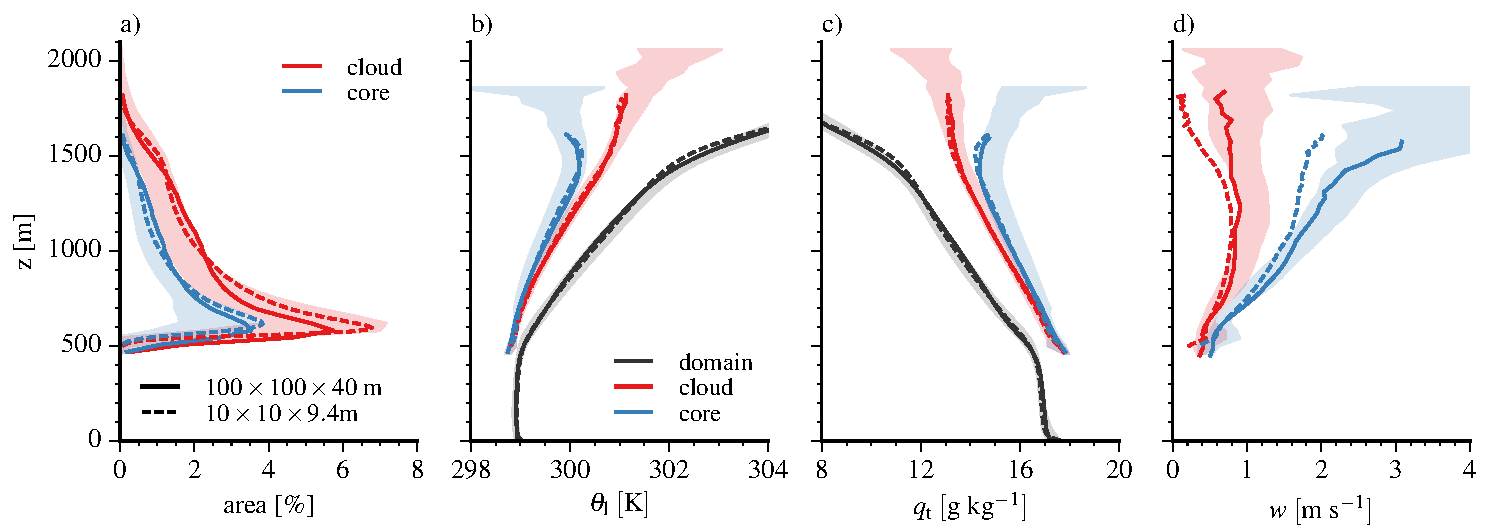
\includegraphics[width=16.6cm]{figs/gmd_bomex_profs.pdf}
	\end{center}
	\caption{BOMEX LES intercomparison (S03). Shown are the domain mean, and conditionally sampled cloud ($q_\mathrm{l} > 0$) and cloud core ($q_\mathrm{l}>0 \ \mathrm{and} \ b-\langle b \rangle > 0$) vertical profiles of (a) area coverage of cloud and cloud core, (b) liquid water potential temperature, (c) total specific humidity and (d) vertical velocity. The results are averaged over $t$ = 18000 s -- 21600 s. The shaded area denotes the mean $\pm$ one standard deviation of the participating models from S03, the solid and dashed lines the results from MicroHH, using the original (solid) and a higher resolution (dashed) setup.}
	\label{fig:bomex}
\end{figure*}

The simulation is run for 6 hours. Statistics are recorded during the final hour, including conditional statistics for the cloud-covered fields ($q_l > 0$) and for the cloud cores ($q_l > 0$ and $\theta_v > 0$). The vertical profile of area coverage and profiles of horizontally-average liquid water potential temperature $\theta_l$, total water $q_t$, and vertical velocity $w$ are shown in Fig. \ref{fig:bomex}. All mean and conditionally sampled statistics at the original resolution are predominantly within one standard deviation of the ensemble mean of data from all models that participated in S03. The horizontally-averaged vertical velocities in the cloud and cloud core decrease considerably with an increase in resolution.

\subsection{GABLS1}
To evaluate the LES mode for stable atmospheric conditions, the GABLS1 LES intercomparison case \citep{Beare2006} (\texttt{cases/gabls1}) was reproduced. The boundary layer develops in this case from a shallow well-mixed layer into a weakly stable boundary layer, driven by a prescribed negative tendency of the surface temperature over a total integration time of 9 hours. The Boussinesq approximation is used, the advection scheme uses fourth-order accurate interpolations (Eq. \ref{eq:interp4}), and the Smagorinsky subgrid turbulence scheme is set up with a Smagorinsky constant equal to 0.12, and a subgrid turbulent Prandtl number of unity. The experiments are performed at two different resolutions with grid cells of $2$ m and $6.25$ m, and compared to the models which participated in the study of \cite{Beare2006}. 

Figure \ref{fig:gabls} shows the domain and time-averaged (over a period from 28800 to 32400~s) vertical profiles of potential temperature ($\langle \theta \rangle$) and the velocity component ($\langle u \rangle$), and also time series of the boundary layer depth ($z_\mathrm{ABL}$) and friction velocity ($u_*$). At the largest grid spacing of $6.25$ m, it takes approximately 2 hours for the flow to become turbulent, as is evident from the delayed boundary layer growth and abrupt changes in $u_*$. Nonetheless, typical features like the low-level jet (Fig. \ref{fig:gabls}b) are well reproduced, and all statistics are predominantly within the range of results from \cite{Beare2006}. With the grid spacing reduced to 2 m, the flow becomes turbulent nearly instantaneously, but the resulting boundary layer depth and surface friction velocity are on the low side compared to the 5 models from \cite{Beare2006} which were run at this resolution. 

\begin{figure*}[t]
\vspace*{2mm}
\begin{center}
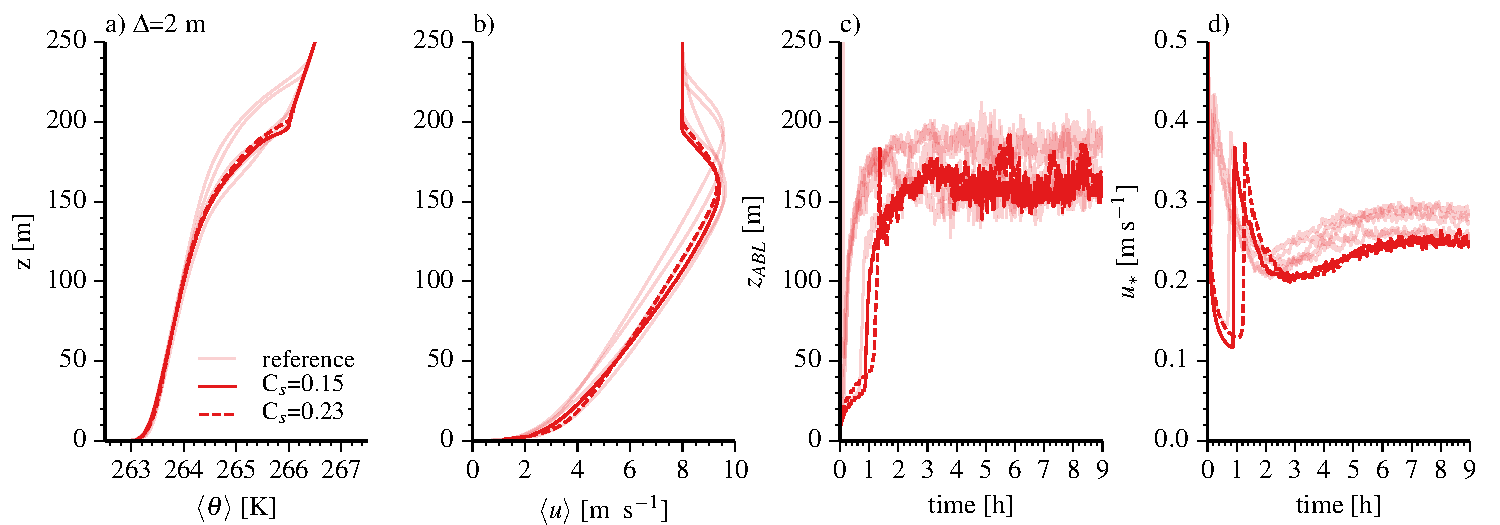
\includegraphics[width=16.6cm]{figs/gmd_gabls_prof_tser.pdf}
\end{center}
\caption{GABLS1 LES intercomparison \citep{Beare2006}. Shown are the vertical profiles of (a) potential temperature and (b) $u$-component of the velocity, and time series of the (c) boundary layer depth and (d) surface friction velocity. The shaded areas show the range in the results from the models that participated in the \citet{Beare2006} study. The dotted black lines show the initial conditions.}
\label{fig:gabls}
\end{figure*}

\section{Performance}\label{sec:performance}
\subsection{CPU}
\begin{figure}[!hbt]
	\vspace*{2mm}
	\begin{center}
		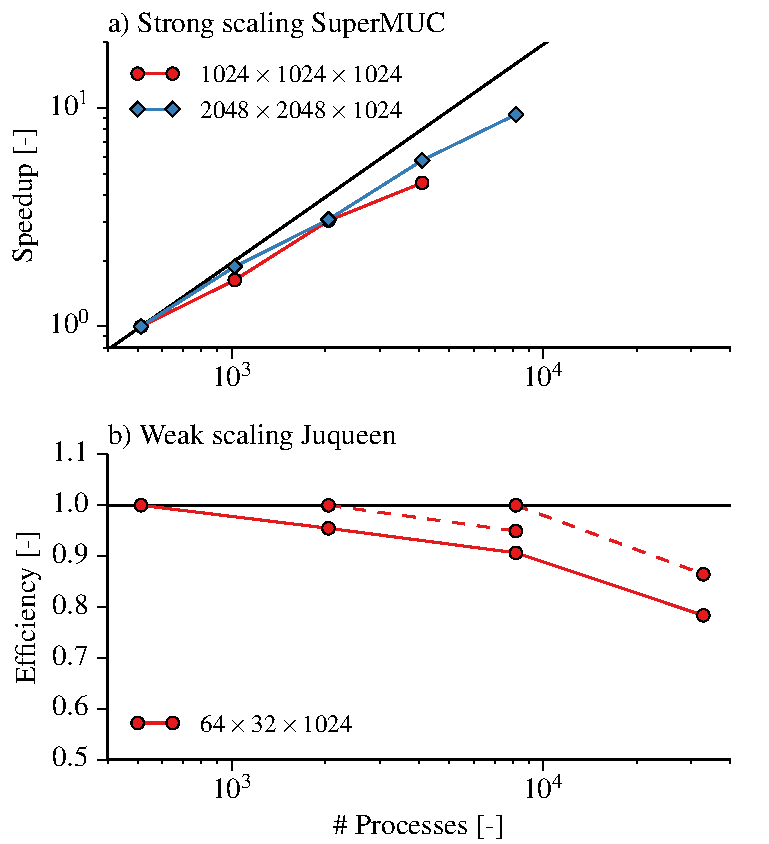
\includegraphics[width=8.3cm]{figs/scaling.pdf}
	\end{center}
	\caption{Speed-up from a strong-scaling experiment (a). Efficiency from a weak-scaling experiments (b). Black lines indicate perfect speed-up and efficiency. The dashed red lines show the efficiency change relative to the previous measurement.}\label{fig:scaling}
\end{figure}
The parallel performance of MicroHH has been evaluated in strong- ($\texttt{cases/strongscaling}$) and weak-scaling\\ ($\texttt{cases/weakscaling}$) experiments. The case used is direct numerical simulation of a buoyancy driven atmospheric boundary layer based on \citet{vanHeerwaarden2014}. For each simulation in the scaling experiments, a series of time steps is performed, and the mean cost per step is calculated over the series. The strong-scaling experiment has been performed on LRZ's SuperMUC\footnote{\url{https://www.lrz.de/services/compute/supermuc/}} machine (experiment was run on the Phase 1 Thin Node 8-core Sandy Bridge-EP Xeon E5-2680 8C, 2 processors per node, Infiniband FDR10 interconnect). In this experiment, simulations were performed on $1024 \times 1024 \times 1024$ and $2048 \times 2048 \times 1024$ grid points, with the number of processes increased throughout the scaling experiment. The weak-scaling experiment has been performed on Forschungszentrum J\"{u}lich's Juqueen\footnote{\url{http://www.fz-juelich.de/ias/jsc/EN/Expertise/Supercomputers/JUQUEEN/JUQUEEN_node.html}} machine (IBM PowerPC A2, 1.6 GHz, 16 cores per node, 5D Torus network, 40 GBps). In this experiment, a fixed $64 \times 32 \times 1024$ grid is assigned to each processor and throughout the experiment the domain size is increased. The results of both experiments are shown in Figure \ref{fig:scaling}.

The strong-scaling experiment shows that increasing the number of processors leads to faster simulations. The speedup is initially close to linear, but each consecutive increase in the number of cores makes the model less efficient. Based on these results, we conclude that for the chosen test case and for the used supercomputers, a work load of approximately $2 \times 10^6$ grid points per core is the best balance between speed and computational efficiency.

The weak scaling shows almost 90 percent efficiency going from 512 to 8192 cores, beyond that the scaling falls off to 80 percent. This can be explained by physical properties of the machine;  beyond 8192 cores a simulation no longer fits on one midplane (a physical unit consisting of 8192 cores), leading to slower communication.

\subsection{Performance GPU (CUDA) implementation}
The GPU implementation of MicroHH allows for fast simulations on a single device. The current state-of-the-art GPUs feature 12~GB of memory, thus simulations of maximally $512 \times 512 \times 512$ grid points of a flow with three velocity components, pressure, two scratch fields for temporary storage, and a single scalar fit in memory. Within this experiment, we compare thus GPU simulations that do not need communication against CPU simulations that require communication between cores and nodes. The reason for doing so, is that nearly all of the presented results in Sections \ref{sec:tests} and \ref{sec:validation_atmos} fit within the memory of a single GPU.

To test the performance of such simulations, the performance of MicroHH on an NVIDIA Quadro K6000 (using CUDA 6.5) has been compared against the Max Planck Institute for Meteorology's cluster Thunder (2 Intel Xeon E5-2670 CPU's per node, 16 cores per node). Three benchmark cases have been chosen: the BOMEX moist convection case on grids of $64^3$, $128^3$, $256^3$ and $512^2 \times 384$, and the channel flow cases of \citet{Moser1999} at a Reynolds-$\tau$ number of 180 and 590.

\begin{table}[t]
	\caption{Speedup of GPU simulation compared to respective CPU simulation performed on $n$ cores.}\label{tab:gpu}
	\begin{tabular}{rccccc}
		\tophline
		case & $n$=1 & $n$=16 & $n$=32 & $n$=64   \\
		\middlehline
		B64  & 18.49 & 1.93 & 1.14 & 0.95 \\
		B128 & 28.01 & 2.98 & 1.51 & 0.92 \\
		B256 & 27.76 & 3.02 & 1.59 & 0.91 \\
		B512 & 29.88 & 3.03 & 1.56 & 0.86 \\
		\middlehline
		M180 & 21.57 & 2.17 & 1.13 & 0.69 \\
		M600 & 22.55 & 2.25 & 1.06 & 0.60 \\
		\bottomhline
	\end{tabular}
\end{table}

The results shown in Table \ref{tab:gpu} point to the great potential of GPU computing. For the considered cases, which all fit on a single GPU, it takes at least 32 cores to reach equal performance. Only at 64 cores, the CPU simulations are notably faster. Therefore, for simulations that fit into its memory, the GPU provides an excellent alternative for the CPU, especially as the GPU is very energy efficient.

\section{Published studies}\label{sec:published}
To date, several studies have been published that make use of MicroHH or data generated with MicroHH. \Citet{vanHeerwaarden2014} studied the scaling of flow over heterogeneously heated land surfaces using DNS and LES, \citet{Gentine2015} used LES to study the structure of the inversion of a convective boundary layer, \citet{vanHeerwaarden2016} developed scaling laws for the convective boundary layer over a surface with a constant temperature from DNS data, \citet{McColl2017} improved surface-layer similarity under mildly convective conditions with the help of DNS data, and \citet{Umphrey2017} used DNS data produced with MicroHH as a reference for their simulations of slope flow.

\section{Future plans}\label{sec:future}
There are several ongoing projects to extend the model. Currently, a parameterization for microphysics has been developed, and an interactive land surface model is under development. In addition, the immersed boundary method following \citet{Tseng2003} is being implemented to allow for simulations of flow over obstacles and hills.

Furthermore, preliminary experiments have been performed to include a Domain-Specific Language (DSL) to enable the expression of complex finite difference operators in simple and compact syntax (\url{https://github.com/Chiil/stencilbuilder/}). This development has shown great potential, for two reasons. First, the DSL prevents implementation errors, as the explicit indexing in computational kernels with spatial operators can be omitted. Second, the DSL allows for simple implementation of system-specific tuning, such as loop tiling or OpenMP.

\conclusions  \label{sec:conclusion} %% \conclusions[modified heading if necessary]
This paper has presented a full description of MicroHH, a new computational fluid dynamics code for simulations of turbulent flows in the atmospheric boundary layer. The governing equations and their implementation has been presented, and a broad validation under a wide range of settings has been shown. MicroHH delivers the expected error convergence of the spatial and temporal schemes, and has proven to be mass, momentum, and energy conserving. The code delivers good performance in weak and strong scaling experiments. Its current limitations are the absense of horizontal boundary conditions other than periodic, and the limited set of available physical parameterizations. Both limitations will be addressed in future versions of the code.

\section{Availability of code and resources}\label{sec:howto}
MicroHH has its own website at \url{http://microhh.org}. The code is hosted at GitHub and can be accessed either via the website, or directly from 
\url{https://github.com/microhh/microhh}. The GitHub website includes a wiki with several tutorials, including one to compile and run the code. The GitHub repository is coupled to Zenodo, which provides DOIs for released software. The release on which the reference paper is based is found at \url{https://zenodo.org/badge/latestdoi/14754940}. A selection of visualizations can be viewed at the MicroHH channel on Vimeo \url{https://vimeo.com/channels/microhh/}.

\appendix \section{Physical constants}
Table \ref{tab:constants} presents an overview of the chosen values for physical constants in the code.
\begin{table*}[t]
\caption{Overview of used constants.}\label{tab:constants}
\begin{tabular}{clcl}
\tophline
Symbol & Description & Value & Units \\
\middlehline
$\kappa$ & Von Karman constant & 0.4 & -\\
$g$ & Gravitational acceleration & 9.81 & $\mathrm{m~s^{-2}}$\\
$c_\mathrm{p}$ & Specific heat of dry air at constant pressure & 1005 & $\mathrm{J~kg^{-1}~K^{-1}}$\\
$p_\mathrm{00}$ & Reference pressure & 1 $\cdot$ 10$^5$ & Pa\\
$R_\mathrm{d}$ & Gas constant for dry air & 287.04 & $\mathrm{J~K^{-1}~kg^{-1}}$\\
$R_\mathrm{v}$ & Gas constant for water vapor & 461.5 & $\mathrm{J~K^{-1}~kg^{-1}}$\\
$L_\mathrm{v}$ & Latent heat of vaporization & 2.5 $\cdot$ 10$^6$ & $\mathrm{J~kg^{-1}}$\\
\bottomhline
\end{tabular}
\end{table*}

\iffalse
\section{Appendix}
\begin{table*}[t]
\caption{Overview of used symbols}\label{tab:symbols}
\begin{tabular}{lll}
\tophline
Symbol & Description & Units \\
\middlehline
$\rho_0$ & Reference density & kg~m$^{-3}$\\
$H_\rho$ & Scale height for density & m\\
$u_i$  & Velocity vector $\left( u, v, w \right)$ & m~s$^{-1}$\\
$x_i$  & Position vector $\left( x, y, z \right)$ & m\\
$p^\prime$ & Perturbation pressure & Pa\\
$p_0$ & Reference pressure & Pa\\
$\rho^\prime$ & Perturbation density & kg~m$^{-3}$ \\
$p^\prime$ & Perturbation pressure & Pa\\
$p_0$ & Reference pressure & Pa\\
$\theta_v^\prime$ & Perturbation virtual potential temperature & K\\
$\theta_{v0}$ & Reference virtual potential temperature & K\\
$g$ & Gravity acceleration & m~s$^{-2}$\\
$\nu$ & Kinematic viscosity & m$^{2}$~s$^{-1}$\\
$\kappa$ & Scalar diffusivity & m$^{2}$~s$^{-1}$\\
$F_i$ & External acceleration vector &  m~s$^{-2}$\\
$S$ & External sources and sinks & variable dependent\\
$\theta$ & Potential temperature & K \\
$\theta_l$ & Liquid water potential temperature & K\\
$b$ & Buoyancy & m~s$^{-2}$\\
$T_0$ & Reference absolute temperature & K\\
$Q$ & Heat input & J~m$^{-3}$~s$^{-1}$\\
$\alpha$ & Slope of surface & rad \\
$N$ & Brunt-Vaissala frequency & s\\
\bottomhline
\end{tabular}
\end{table*}
\fi

\begin{acknowledgements}
Finishing the 1.0 version of MicroHH has only become possible thanks to extensive discussions and exchange of code with many of the developers of DALES (Huug Ouwersloot, Stephan de Roode, Arnold Moene and Jordi Vil\`{a}-Guerau de Arellano), PALM (Bj\"{o}rn Maronga and Siegfried Raasch), UCLA-LES (Linda Schlemmer and Bjorn Stevens) and ICON (Leonidas Linardakis). We thank Alan Shapiro for the discussions on the bottom boundary condition for pressure for buoyancy driven flows and for his comments on the manuscript. We thank Elie Bou-Zeid and an anonymous reviewer for their constructive comments on the manuscript. The authors gratefully acknowledge the Gauss Centre for Supercomputing (GCS) for providing computing time for a GCS Large-Scale Project on the GCS share of the supercomputer JUQUEEN at J\"{u}lich Supercomputing Centre (JSC). 
\end{acknowledgements}

\bibliographystyle{copernicus}
\bibliography{../../misc/refs}
%\bibliography{microhharticle}

\end{document}
